% Szglab4
% ===========================================================================
%
% 
% Szglab4
% ===========================================================================
%
\documentclass[11pt,oneside]{scrbook}

\usepackage[utf8]{inputenc}
\usepackage[T1]{fontenc}

\usepackage{fancyhdr}

\usepackage[magyar]{babel}

\usepackage{longtable}

\usepackage[usenames]{color}

\usepackage{float}

\usepackage{times}

\usepackage{listings}

\usepackage{includes/szglab4}

\usepackage[%
	pdftitle={Szglab 4},% A PDF dokumentum címe.
	pdfauthor={X.Y.)},% Szerző(k) neve(i)
	pdfsubject={Szglab 4},% A PDF dokumentum témája
	pdfcreator={MiKTeX, LaTeX with hyperref and KOMA-Script}, % A PDF dokumentum készült ...
	pdfkeywords={Szglab4},% Kulcsszavak
	pdfpagemode=UseOutlines,% Tartalomjegyzék megjelenítése megnyitáskor
	pdfdisplaydoctitle=true,% Fájlnév helyett a dokumentum neve jelenjen meg
	pdflang=hu,% A dokumentum nyelve
	unicode
]{hyperref}

\definecolor{LinkColor}{rgb}{0,0,0}
\definecolor{ListingBackground}{rgb}{1,1,1}

\hypersetup{%
	colorlinks=true,% Színes linkek aktiválása a dokumentumban (keretek nélkül)
	linkcolor=LinkColor,%    szín beállítása
	citecolor=LinkColor,%    szín beállítása
	filecolor=LinkColor,%    szín beállítása
	menucolor=LinkColor,%    szín beállítása
	urlcolor=LinkColor,%     URL hivatkozások színe
	bookmarksnumbered=true
}

%
% ===========================================================================
% EOF
%


\graphicspath{ {images/} }

%
\csapat{\team}{40}
\konzulens{Szabó Ádám Imre}
\taga{Kovács Levente Ákos}{CM6UKU}{vazul250@gmail.com }
\tagb{Lovász Attila Bence}{INCMI7}{attonet2@gmail.com }
\tagc{Graics Vince}{HY9XQ6}{wince17@gmail.com}
\tagd{Magyar Milán Bertalan}{MCDNQL}{milangfx@gmail.com}
\tage{Tóth Krisztián Dávid}{J38GIK}{tht.krisztian@gmail.com}
\datum{\today}
%
\begin{document}
%
% Nem aktuális sorokat kommentezni
%
%\fedlap{3. Analízis modell kidolgozása 1}
%\fedlap{4. Analízis modell kidolgozása 2}
%\fedlap{5. Szkeleton tervezése}
\fedlap{6. Szkeleton beadása}
%
% Tartalomjegyzék és ábrák jegyzéke
%
\clearpage \tableofcontents \pagestyle{fancy}
%\clearpage \listoffigures \pagestyle{fancy}
%
% Nem aktuális fejezetek kikommentezve
%
%\setcounter{chapter}{1}
%% Szglab4
% ===========================================================================
%
\chapter{Követelmény, projekt, funkcionalitás}

\thispagestyle{fancy}

\section{Bevezetés}

\subsection{Cél}

A project követelményeinek, alapvető felépítésének és funkcionalitásának ismertetése, ezek segítségével a fejlesztési folyamatok majd a végleges program felépítésének megtervezése. Fejlesztés közben ezeket figyelembe kell majd venni és tőlük eltérni nem szabad.

\comment{A dokumentum célja.}

\subsection{Szakterület}
A project a Szoftver laboratórium 4. tantárgy feladatának megoldására született. Az elkészítendő szoftver egy számítógépes játék, nem kimondottan egy szakterület részére készül, inkább szórakoztatás céljából.

\comment{A kialakítandó szoftver milyen területen használható, milyen célra.}

\subsection{Definíciók, rövidítések}
\begin{itemize}
\item 
\end{itemize}
\comment{A dokumentumban használt definíciók, rövidítések magyarázata.}

\subsection {Hivatkozások}
Szoftver Labor 4 - \url{https://www.iit.bme.hu/~szoftlab4/}

\comment{A dokumentumban használt anyagok, web-oldalak felsorolása}

\subsection{Összefoglalás}
A dokumentum további részeiben található:
\begin{itemize}
\item 2.2 Áttekintés: A project terveinek, funkcióinak áttekintése, a felhasználók lehetőségeinek áttekintése
\item 2.3 Követelmények: A project során elvárt követelmények kidolgozása, külön kitérve funkcionális, erőforrás, átadással kapcsolatos és egyéb nem funkcionális követelményekre.
\item 2.4 Lényeges use-case-ek felsorolása, use-case diagram
\item 2.5 Szótár: A project során bevezetett fogalmak körülírása.
\item 2.6 Project terv: A project résztvevőinek feladatkörei és határidők részletes kifejtése
\item 2.7 Napló: Az elvégzett feladatok és ráfordított idő felsorolása
\end{itemize}

\comment{A dokumentum további részeinek rövid ismertetése}

\pagebreak
\section{Áttekintés}
\subsection{Általános áttekintés}
\begin{itemize}
\item játékmotor
\item director
\item HUD
\item játék menü
\item garfikus felület
\item pályák
\item robotok
\end{itemize}
\\A szoftver fontos eleme a Játékmotor. Ez teremti meg a kezdeti feltételeket és irányítja a játék folyását. Ez fogja ellenőrizni, hogy a robotok leesnek-e a pályáról, ha olajfoltba lépnek letiltja az irányítást a játékos oldalon, illetve ha ragacsba lép egy játékos, akkor lelassuljon. A Játékmotor indulása előtt lekéri a Pályák alrendszertől a kiválasztott pályát.
\\A director alrendszer feladata az idő léptetése, másodpercenként ugranak a robotok ezt ütemezi.
\\A HUD alrendszer hivatott jelezni, hogy a játékos számára elérhető-e a olaj vagy ragacskészlet \comment{,továbbá a megtett körök számát}
\\A játék menü alrendszer feladata a játék során a megfelelő parancsra megállítani a játékot és a beállítások (pl.: grafikai, hang) állíthatósága.
\\A grafikus felület feladata, hogy kapcsolatot létesítsen a játékossal vizuális információkkal és a játékos ezen keresztül irányíthatja a játékmotort.
\\A Pályák alrendszer betölti a Pályafájlokból a pályákat, tárolja, majd azokat a Játékmotor rendelkezésére bocsájtja.
\\A Robotok alrendszer betölti a robotokat a Robotfájlokból, tárolja azokat, majd a Játékmotor rendelkezésére bocsájtja.
\\Hálózatot a szoftver nem igényel. Háttértáron pedig a program .jar archívumainak, a kirajzoláshoz szükséges pálya és robot képeknek, a pályákat tartalmazó fájloknak szükséges helyet biztosítani. Ezeken kívül nincs szükség futás idejű tárhelyigényre. 

\comment{A kialakítandó szoftver legmagasabb szintű architekturális képe. A fontosabb alrendszerek felsorolása, a közöttük kialakítandó interfészek lényege, a felhasználói kapcsolatok alapja. Esetleges hálózati és adattárolási elvárások.}

\subsection{Funkciók}
\comment{A feladat kb. 4000 karakteres (kb 1,5 oldal) részletezettségű magyar nyelvű leírása. Nem szerepelhetnek informatikai kifejezések.}

\subsection{Felhasználók}
A játék 2 játékos módban indíthat. A játékosnak semmiféle előképzettségre nincs szüksége, a játék menete gyorsan elsajátítható. A játékban nem lesz pályaszerkesztő. A játékot nem lehet elmenteni, mindig újból kell kezdeni.
\comment{A felhasználók jellemzői, tulajdonságai}

\subsection{Korlátozások}
A BME IIT Szoftver Laboratórium tantárgy oktatói (a megrendelők) által kiírt specifikáció megköveteli, hogy a program a HSZK gépein a beadások alkalmával futtathatók legyenek. Ezekre a gépekre már előre feltelepített JRE 1.7-es környezet elérhető, ezért csak a JDK 1.7-es verziójaban már létező függvények, osztályok használhatóak a kód megírása során.
\comment{Az elkészítendő szoftverre vonatkozó – általában nem funkcionális - előírások, korlátozások.}

\subsection{Feltételezések, kapcsolatok}
\comment{A dokumentumban használt anyagok, web-oldalak felsorolása}

\section{Követelmények}
\subsection{Funkcionális követelmények}
Prioritások:
\begin{itemize}
\item alapvető
\item fontos
\item opcionális
\end{itemize}
Források:
\begin{itemize}
\item specifikáció
\item csapat
\item konzulens
\end{itemize}

\comment{Az alábbi táblázat kitöltésével készítendő. Dolgozzon ki követelmény azonosító rendszert! Az ellenőrzés módja szokásosan bemutatás és/vagy kiértékelés. Prioritás lehet alapvető, fontos, opcionális. Az alapvető követelmények nem teljesítése végzetes. Forrás alatt a követelményt előíró anyagot, szervezetet kell érteni. Esetünkben forrás lehet maga a csapat is, mikor ő talál ki követelményt. Use-case-ek alatt az adott követelményt megvalósító használati esete(ke)t kell megadni.}

% Azonosító, Leírás, Ellenőrzés, Prioritás, Forrás, Use-case, Komment
\begin{longtable}{| l | l | l | l | l | l | l |}
\hline
\textbf{Azonosító}   & \textbf{Leírás} & \textbf{Ellenőrzés} & \textbf{Prioritás} & \textbf{Forrás} & \textbf{Use-case} & \textbf{Komment} \tabularnewline
\hline 1.01 & Játék menü & & alapvető & & &\tabularnewline
\hline 1.02 & Beállítások kezelése & & alapvető & & &\tabularnewline
\hline 1.03 & Játék elindítása & & alapvető & & &\tabularnewline
\hline 1.04 & Pályáról leesők kiesnek & & alapvető & & &\tabularnewline
\hline 1.05 & Előre elkészített versenypálya & & alapvető & & &\tabularnewline
\hline 1.06 & \vtop{\hbox{\strut Robotok a kezdőpozíciójukból}\hbox{\strut indulnak}}  & & alapvető & & &\tabularnewline
\hline 1.07 &\vtop{\hbox{\strut Pályán vannak olajfoltok és}\hbox{\strut ragacsfoltok}}   & & alapvető & & &\tabularnewline
\hline 1.08 &\vtop{\hbox{\strut Robotok fel vannak szerelve }\hbox{\strut olaj és ragacskészlettel}}  & & alapvető & & &\tabularnewline
\hline 1.09 &\vtop{\hbox{\strut 2 személy tudjon játszani}\hbox{\strut egyszerre}} & & alapvető & & &\tabularnewline
\hline 1.10 & \vtop{\hbox{\strut USB-s joystickkal}\hbox{\strut vezérelhető robotok}} & & opcionális & & &\tabularnewline
\hline
\end{longtable}

\subsection{Erőforrásokkal kapcsolatos követelmények}

\comment{A szoftver fejlesztésével és használatával kapcsolatos számítógépes, hardveres, alapszoftveres és egyéb architekturális és logisztikai követelmények}

% Azonosító, Leírás, Ellenőrzés, Prioritás, Forrás, Komment
\begin{longtable}{| l | l | l | l | l | l |}
\hline
\textbf{Azonosító}   & \textbf{Leírás} & \textbf{Ellenőrzés} & \textbf{Prioritás} & \textbf{Forrás} & \textbf{Komment} \tabularnewline
\hlie
\hline 2.01 & JRE  & bemutatás  & alapvető  & megrendelő & Java IDE  \tabularnewline
\hline 2.02 & Eclipse & nincs & opcionális & csapat & Java IDE \tabularnewline
\hline 2.03 & NetBeans IDE & nincs  & opcionális  & csapat  & Java IDE  \tabularnewline
\hline 2.04 & IntelliJ IDEA & nincs  & opcionális  & csapat  & Java IDE  \tabularnewline
\hline 2.05 & ShareLatex & nincs  & opcionális  & csapat  & online LaTeX editor  \tabularnewline
\hline 2.06 & Git & nincs  & alapvető  & csapat  & Elosztott verziókezelő \tabularnewline
\hline 2.07 & GitHub account & nincs  & alapvető & csapat & Git tárhely \tabularnewline
\hline 2.08 & PC & bemutatás  & alapvető  & megrendelő  &  \tabularnewline
\hline 2.09 & Monitor & nincs  & alapvető  & csapat  &  \tabularnewline
\hline 2.10 & Billentyűzet & nincs  & alapvető  & csapat  &  \tabularnewline
\hline 2.11 & Egér & nincs  & alapvető  & csapat  &  \tabularnewline
\hline 2.12 & Google Calendar & nincs  & opcionális  & csapat  & Naptár alkalmazás \tabularnewline
\hline 2.13 & Google Mail & nincs  & opcionális  & csapat  & Levelező rendszer \tabularnewline
\hline 2.14 & Sympa levelezőlista & nincs  & opcionális  & csapat & \url{lists.sch.bme.hu}  \tabularnewline
\hline 2.15 & Doxygen  & nincs  & opcionális  & csapat & Programozói dokumentáció 
\hline
\end{longtable}


\subsection{Átadással kapcsolatos követelmények}
\comment{A szoftver átadásával, telepítésével, üzembe helyezésével kapcsolatos követelmények}

% Azonosító, Leírás, Ellenőrzés, Prioritás, Forrás, Komment
\begin{longtable}{| l | l | l | l | l | l |}
\hline
\textbf{Azonosító}   & \textbf{Leírás} & \textbf{Ellenőrzés} & \textbf{Prioritás} & \textbf{Forrás} & \textbf{Komment} \tabularnewline
\hline
\hline 3.01 & Szkeleton átadás & bemutatás  & alapvető  & megrendelő  & márc. 23  \tabularnewline
\hline 3.02 & Prototípus átadás & bemutatás & alapvető & megrendelő  & ápr. 20  \tabularnewline
\hline 3.03 & Teljes program átadása  & bemutatás  & alapvető & megrendelő & máj. 15  \tabularnewline
\hline 3.04 & \vtop{\hbox{\strut Útmutató alapján}\hbox{\strut telepíthető, indítható}}  & bemutatás  & fontos  & megrendelő  &   \tabularnewline
\hline 3.06 &\vtop{\hbox{\strut A programnak működnie}\hbox{\strut kell a BME HSZK számítógépein}} & bemutatás & alapvető & megrendelő &  \tabularnewline
\hline
\end{longtable}

\subsection{Egyéb nem funkcionális követelmények}
Nincs egyéb nem funkcionális követelmény.
\comment{A biztonsággal, hordozhatósággal, megbízhatósággal, tesztelhetőséggel, a felhasználóval kapcsolatos követelmények}

% Azonosító, Leírás, Ellenőrzés, Prioritás, Forrás, Komment
%\begin{longtable}{| l | l | l | l | l | l |}
%\hline
%\textbf{Azonosító}   & \textbf{Leírás} & \textbf{Ellenőrzés} & \textbf{Prioritás} & \textbf{Forrás} & \textbf{Komment} \tabularnewline
%\hline\hline ... & ... & ... & ... & ... & ... \tabularnewline
%\hline
%\end{longtable}


\section{Lényeges use-case-ek}
\comment{A 2.3.1-ben felsorolt követelmények közül az alapvető és fontos követelményekhez tartozó használati esetek megadása az alábbi táblázatos formában.}
\subsection{Use-case leírások}

\comment{Minden use-case-hez külön}

\usecase{...}{...}{...}{...}

\usecase{...}{...}{...}{...}

\section{Szótár}
\begin{itemize}
\item 
\end{itemize}
\comment{A szótár a követelmények alapján készítendő fejezet. Egy szótári bejegyzés definiálásához csak más szótári bejegyzések és köznapi – a feladattól független – fogalmak használhatók fel. A szótár mérete kb. 1-2 oldal legyen.}

\section{Projekt terv}
\subsection{Csapat}
A csapat 5 főből áll. A következő táblázat a személyes preferenciákat tartalmazza, a feladatokat úgy osztjuk ki, hogy közel azonos nehézségűek legyenek, miközben ezeket a preferenciákat szem előtt tartjuk.

\subsection {Kommunikáció}

\subsection{Használt programok}

\subsection{Mérföldkövek, határidők}
\
\comment{Tartalmaznia kell a projekt végrehajtásának lépéseit, a lépések, eredmények határidejét, az egyes feladatok elvégzéséért felelős személyek nevét és beosztását, a szükséges erőforrásokat, stb. Meg kell adni a csoportmunkát támogató eszközöket, a választott technikákat! Definiálni kell, hogy hogyan történik a dokumentumok és a forráskód megosztása!}



%% Szglab4
% ===========================================================================
%
\pagebreak
\section{Napló}

\begin{naplo}

\bejegyzes
{2015.02.16.~16:30~} % Kezdet
{1 óra} % Időtartam
{Kovács\newline
Lovász\newline
Tóth\newline
Graics\newline
Magyar
} % Résztvevők
{Kezdeti megbeszélés. Specifikáció körvonalazása. Lehetséges use-case-ek átbeszélése. Feladatok kiosztása} % Leírás

\bejegyzes
{2015.02.16.~20:15~}
{1,5 óra}
{Tóth}
{Tevékenység: Specifikáció készítés}

\bejegyzes
{2015.02.17.~17:00~}
{1 óra}
{Lovász\newline
Kovács}
{Tevékenység: Lehetséges Use-Case-ek megalkotása, Use-Case Diagramm elkészítése}

\bejegyzes
{2015.02.17.~20:30~}
{1,5 óra}
{Graics}
{Tevékenység: Funkcionalitás megírása}

\bejegyzes
{2015.02.18.~8:15~} % Kezdet
{1 óra} % Időtartam
{Kovács\newline
Lovász\newline
Tóth\newline
Graics\newline
Magyar
} % Résztvevők
{Funkcionalitások átbeszélése, mérlegelés. Feladatok kiosztása}


\bejegyzes
{2015.02.19~18:00~}
{2 óra}
{Magyar}
{Tevékenység: Szótár megalkotása}

\bejegyzes
{2015.02.19~21:00~}
{2 óra}
{Graics}
{Tevékenység: Definíciók és rövidítések megalkotása}

\bejegyzes
{2015.02.22.~14:00~}
{0,5 óra}
{Tóth}
{Tevékenység: Dokumentáció végső simításai}

\end{naplo}

%\setcounter{chapter}{2}
%% Szglab4
% ===========================================================================
%
\chapter{Analízis modell kidolgozása 1}

\thispagestyle{fancy}

\section{Objektum katalógus}

\subsection{Glue}
A „Glue” objektum megvalósít egy adott tulajdonságú akadályt. Amely robot belemegy, annak a sebességét megfelezi. 
\subsection{GUI}
A grafikus felületet megvalósító objektum. Ez az objektum maga a menü ami a játék indítása után ugrik fel, itt találhatóak a beállítások (mint például a gondolkodás idő és a maximális játék idő vagy a körök száma) és a játékmódok. Gombnyomásra fogja elindítani a játék működési szálát. Ez az objektum kezeli az ablak eseményeit és a játék bezárását.
\subsection{HUD}
Ez az objektum követi és nyilvántartja, hogy a robotok hány checkpoint-on mentek át, mennyi olaj és ragacs van náluk amit felhasználhatnak, illetve kiírja a képernyőre a hátramaradó időt és a megtett körök számát. Feladata, hogy minden körben megvizsgálja, hogy a robotok elérték-e a következő checkpointot.
\subsection{MapBuilder}
Fájlból beolvassa és létrehozza a memóriában a pályát, a kezdő pozíciókat és a checkpointokat reprezentáló objektumokat.  Mivel a  MapBuilder objektum tárolja a pályát így feladat, hogy vizsgálja a robotok azon belül tartózkodását.  
\subsection{Obstacle}
Az Obstacle absztrakt osztály, mely a Unit osztályból származik le. Ez az osztály fogja összefogni a pályán található (lerakott) akadályokat és bevezet egy absztrakt függvényt, ami a leszármazottakban implementálva érvényesíti hatását (lassítás, csúszás) egy robotra.
\subsection{Oil}
Ez az objektum az Obstacle osztály leszármazottja. Hasonlóan a Glue objektumhoz, egy adott hatást valósít meg, ami letiltja a következő körben történő irányítását a robotnak, ami belelépett.
\subsection{Phoebe}
A játék logikát megvalósító objektum. Listában tárolja a pályán tartózkodó robotokat, akadályokat és figyeli, hogy mikor ér véget a játék. A „Phoebe” objektumrajzolja ki az objektumokat a pályán és szálként indítható osztályt, melyben maga a játék fut. Játékindításkor berakja a pályára a robotokat és az akadályokat a kezdő pozíciókba. Ebben az objektumbantörténnek az ellenőrzések (akadályba vagy robotba ütközések, pályáról leesés).
\subsection{Robot}
Olyan objektum, mely a pályán található robotokat valósítja meg. Leírja a viselkedésüket és a kezelésüket. A „Robot” osztály a Unit-ból származik le, ezáltal van pozíciója és az ütközés is le van kezelve. Felelős a mozgásért, megállapítja egy adott akadállyal vagy robottal ütközött-e és kezeli a felhasználó által leütött gombokat.

\subsection{Timer}
Az eltelt időt és a fennmaradt idő nyilvántartásáért felelős. Ilyen például a játék elején három másodperces visszaszámlálás vagy a időlimites játékmód esetén, amikor a maximális időtől számol visszafelé. 
\subsection{Unit}
A Unit absztarkt osztály a pályán található objektumoknak a szülőosztálya. Tárolja a pozíciót, egy sokszöget, amivel vizsgálható az ütközés és a pályán megjelenő képüket. Továbbá ez az osztály valósítja meg a függvényt, ami ellenőrzi azt, ha két Unit ütközik (robotok egymással, robot akadállyal).


\section{Osztályok leírása}

\subsection{Glue}
\begin{itemize}
\item Felelősség\\
A játékban szereplő Ragacs foltok viselkedését leíró osztály
\item Ősosztályok\\
Unit$\rightarrow$Obstacle
\item Metódusok
	\begin{itemize}
		\item void \textbf{effect}(Robot r): Ütközéskor hívja meg az ütközést vizsgáló függvénye a Robot osztálynak. Módosítja a robot slowed értékét a 50\%-ra a robot slowed attribútum setterének meghívásával.
	\end{itemize}
\end{itemize}

\subsection{GUI}
\begin{itemize}
\item Felelősség\\
A grafikus felületért felelős osztály, mely a menüt és a játékot megjeleníti.
\item Attribútumok
	\begin{itemize}
		\item \textbf{Phoebe} game: referencia a játékra
	\end{itemize}
\item Metódusok
	\begin{itemize}
		\item\textbf{GUI}(): Konstruktor. Beállítja az ablak nevét, létrehozza az ablak elemeit, elrendezi őket és beállítja a figyelőket(ActionListener).
	\end{itemize}
\end{itemize}

\subsection{HUD}
\begin{itemize}
\item Felelősség\\
A robotok ragacs- és olajkészletét, illetve megtett köreit és checkpontjait számolja. Megvalósítja a checkpoint ellenőrzést.
\item Attribútumok
	\begin{itemize}
		\item \textbf{int[]} checkpointReached: Minden robothoz külön tárolja a legutoljára érintett checkpoint sorszámát.
		\item \textbf{int[]} lap: Minden robothoz tárolja a megtett körök számát. 
		\item \textbf{int[]} numGlue: Minden robothoz tárolja a ragacsok számát.
		\item \textbf{int[]} numOil: Minden robothoz tárolja az olajok számát.
		\item \textbf{List<Shape>} checkpoints: Tárolja a checkpointokat reprezentáló objektumokat List adatszerkezetben. A checkpointSearch függvény kérdezi le ebből a következő checkpoint helyzetét. 
		\item \textbf{List<Robot>} robots: A robotokat tároló List adatszerkezet. A checkpointSearch függvény kérdezi le ebből a robotokat, majd azok helyzetét.
	\end{itemize}
\item Metódusok
	\begin{itemize}
		\item \textbf{HUD}(List<Robot> robs): Konstruktor, inicializálja a köröket számláló változót, az érintett checkpointokat, a ragacs és olajkészleteket. 
		\item void \textbf{checkpointSearch}(): Ellenőrzi hogy a robotok teljesítették-e a következő checkpointot.
		\item void \textbf{setCheckpoints}(List<Shape> checkObj): Checkpointokat reprezentáló adatszerkezet betöltése.
		
	\end{itemize}
\end{itemize}

\subsection{MapBuilder}
\begin{itemize}
\item Felelősség\\
A pálya felépítéséért, a checkpointok tárolásáért és a robot pályán tartózkodásának vizsgálatáért felelős osztály.
\item Attribútumok
	\begin{itemize}
		\item \textbf{Shape} map: A pályát reprezentáló objektum. 
		\item \textbf{List<Shape>} checkpoints: Tárolja a checkpointokat reprezentáló objektumokat List adatszerkezetben.
		\item \textbf{int[]} startPosPlayerOne: Meghatároz egy (x,y) koordinátát, ahol az első játékos kezd.
		\item \textbf{int[]} startPosPlayerTwo: Meghatároz egy (x,y) koordinátát, ahol az második játékos kezd.
	\end{itemize}
\item Metódusok
	\begin{itemize}
		\item \textbf{MapBuilder}(): Konstruktor, a pálya beolvasása fájlból, majd létrehozása.
		\item boolean \textbf{fallingDown}(Shape othershape): Igaz értéket ad vissza, ha a robot leesett a pályáról, hamisat ha még rajta van.
	\end{itemize}
\end{itemize}

\subsection{Obstacle}
\begin{itemize}
\item Felelősség\\
A pályán/játékosoknál lévő különböző akadályokat (ragacs,olaj) összefogó ősosztály.
\item Ősosztályok\\
Unit
\item Attribútumok
	\begin{itemize}
		\item \textbf{int} WIDTH: Az akadályokat jellemző szélesség. Szükség van rá, hogy létrehozzuk a leszármazottak hitbox-át(sokszög pályaelem).
		\item \textbf{int} HEIGHT: Az akadályokat jellemző hosszúság. Szükség van rá, hogy létrehozzuk a leszármazottak hitbox-át(sokszög pályaelem).
	\end{itemize}
\item Metódusok
	\begin{itemize}
		\item \textbf{Obstacle}(int x, int y, String imagelocation): meghívja a Unit konstruktorát a megadott adatokkal és létrehoz egy sokszög elemet ami reprezentálja a pályán majd.
		\item void \textbf{effect}(Robot r): Meghatározza, milyen hatással van a robotra, ha érintkezik egy Obstacle-lel. Absztrakt.
	\end{itemize}
\end{itemize}

\subsection{Oil}
\begin{itemize}
\item Felelősség\\
A pályára lerakható olaj megvalósítása. Ha belelép egy játékos egy ilyen olajfoltba az effect függvény letiltja a mozgatást az adott roboton a következő ugrásig.
\item Ősosztályok\\
Unit $\rightarrow$ Obstacle 
\item Metódusok
	\begin{itemize}
		\item \textbf{Oil}(int x, int y, String imagelocation): Egy Oil elem létrehozásáért felelős.
		\item void \textbf{effect}(Robot r): Meghatározza, milyen hatással van a robotra, ha beleugrik egy olajfoltba. Ebben az esetben letiltja a játékost, hogy irányt váltson.
	\end{itemize}
\end{itemize}

\subsection{Phoebe}
\begin{itemize}
\item Felelősség\\
A játék motorját képviselő osztály. A robotok pozíciójáért, az akadályok elhelyezéséért és a játék végéért felel.
\item Attribútumok
	\begin{itemize}
		\item \textbf{boolean} ended: Állapot változó, ha vége a játéknak, akkor true. Ha beteljesül egy játék végét jelentő esemény, akkor ezen a változón keresztül leáll a játék és megállapítódik a nyertes.
		\item \textbf{List<Robot>} robots: A játékban szereplő robotok listája.
		\item \textbf{List<Obstacle>} obstacles: A játékban szereplő akadályok listája.
		\item \textbf{HUD} hud: A játékosok előrehaladását, ragacs és olajkészleteit tartja számon
		\item \textbf{MapBuilder} map: 
	\end{itemize}
\item Metódusok
	\begin{itemize}
		\item \textbf{Phoebe}(Setting set): A játék felépítése, a robotok lista, az akadályok lista létrehozása
		\item void \textbf{run}(): Ez a metódus futtatja a főciklust, amelyben maga a játék működik.
	\end{itemize}
\end{itemize}

\subsection{Robot}
\begin{itemize}
\item Felelősség\\
A játékban résztvevő robotok viselkedését és kezelését leíró osztály.
\item Ősosztályok\\
Unit
\item Interfészek\\
Nincs interfésze
\item Attribútumok
	\begin{itemize}
		\item \textbf{int} staticID: Az osztályhoz tartozó statikus azonosító, a példány                azonosítójának(id) meghatározásához szükséges.
		\item \textbf{int} HEIGHT: A robot képének magassága, collision                      detektálásnál, továbbá az irányítást segítő nyíl kezdő koordinátájának                  meghatározásánál szükséges.
		\item \textbf{int} WIDTH:A robot képének szélessége, funkcionalitásban hasonló a WIDTH-hez.
		\item \textbf{int} ID: A robot példányának egyedi azonosítója, a keyconfig sorának                     indexelésére és a collison detektálásnál az önmagával való ütközés                      kivédésére szükséges.
		\item \textbf{double} slowed: A sebesség modosításáért felel, default értéje 1.0, amennyiben ragacsba lép a robot ez 0.5-re módosul és minden ugrás végén visszaáll az eredeti értékére, ugrásnál ezzel szorozzuk be a végkordinátát kiszámító sugár hosszát.
		\item \textbf{boolean} oiled: Azt jelzi, hogy olajba lépett-e, ennek hatására a mozgás iránya módosíthatatlanná válik egy kis időre. 
		\item \textbf{int} arrowendx: A robot irányítását segítő nyilnak az x koordinátája, a nyíl kirajzolásánál van szerepe.
		\item \textbf{int} arrowendy: A robot irányítását segítő nyilnak az y koordinátája, a nyíl kirajzolásánál van szerepe.
		\item \textbf{double} alpha: A robot irányítását segítő nyíl vízszintessel bezárt szöge. A nyil kirajzolásánál, az ugrás végpontjának meghatározánál van szerepe.
		\item \textbf{boolean} moved: Azt jelöli, hogy lépett-e már a robot az aktuális körben. A megjelenítésnél(nyilat ugrás közben nem jelenítjük meg),illetve az irányítás letiltásánál van szerepe(olajba lépés esetén).
		\item \textbf{int[][]} keyconfig: A játékosok írányítását tároló mátrix. A játékosok irányítását ennek segítségével határozzuk meg a keyPressed függvénybe. A sor meghatározza a felhasználóhoz tartozó gombokat, az oszlopok a funkciók(olaj/ragacs lerakás, a nyíl jobbra/balra mozgatása)
\end{itemize}
\item Metódusok\\
	\begin{itemize}
		\item \textbf{Robot}(int x,int y,String imagelocation,Phoebe p): Létrehoz egy robotot a megadott x,y kordinátákon, betölti a képét az imagelocation cím alapján, továbbá eltárolja a játékmotor referenciáját.
		\item \textbf{void deathanimation}():A Robot halálának gafikus megjelenítéséért felelős függvény.
		\item boolean \textbf{collisionWithObstacle}(Obstacle o): Ellenőrzi hogy a robot ütközött-e az akadállyal, igazzal tér vissza ha igen, hamissal ha nem.
		\item boolean \textbf{collisionWithRobot}(Robot r): Ellenőrzi hogy a robot ütközött-e másik robottal , igazzal tér vissza ha igen, hamissal ha nem. ID alapján kiszüri ha önmagára hívják meg.
		\item void \textbf{keyPressed}(Keyevent e):A robot irányítását megvalósító függvény, a játékmotor keylistener-e által hívódik meg, a lenyomott billentyű keyevent-jére. A következő ugrás beállítása, a ragacs/olaj lerakása történhet itt. A keyconfig változó felhasználásával.
	\end{itemize}
\end{itemize}

\subsection{Timer}
\begin{itemize}
\item Felelősség\\
A visszaszámlálásért (idő, director time) felelős.
\item Metódusok
	\begin{itemize}
		\item \textbf{Timer}(int i): Konstruktor, inicializál egy viszaszámláló órát.
		\item boolean \textbf{isZero}(): Igazzal tér vissza ha a megadott idő lejárt;
	\end{itemize}
\end{itemize}

\subsection{Unit}
\begin{itemize}
\item Felelősség\\
A pályán található objektumokért felel és azok viszonyáról (például ütközésükről).
\item Attribútumok
	\begin{itemize}
		\item \textbf{int} x: Az egység x koordinátája
		\item \textbf{int} y: Az egység y koordinátája
		\item \textbf{Rectangle} hitbox: Az egységet a pályán reprezentáló sokszög.
	\end{itemize}
\item Metódusok
	\begin{itemize}
		\item void \textbf{move}() : Absztrakt függvény, mely a leszármazottakban fog megvalósulni. Az egységek mozgásáért felelős.
		\item boolean \textbf{intersect}(Unit u): Két egység ütközését meghatározó függvény.
	\end{itemize}
\end{itemize}
\pagebreak
\section{Statikus struktúra diagramok}

\begin{figure}[h]
\begin{center}
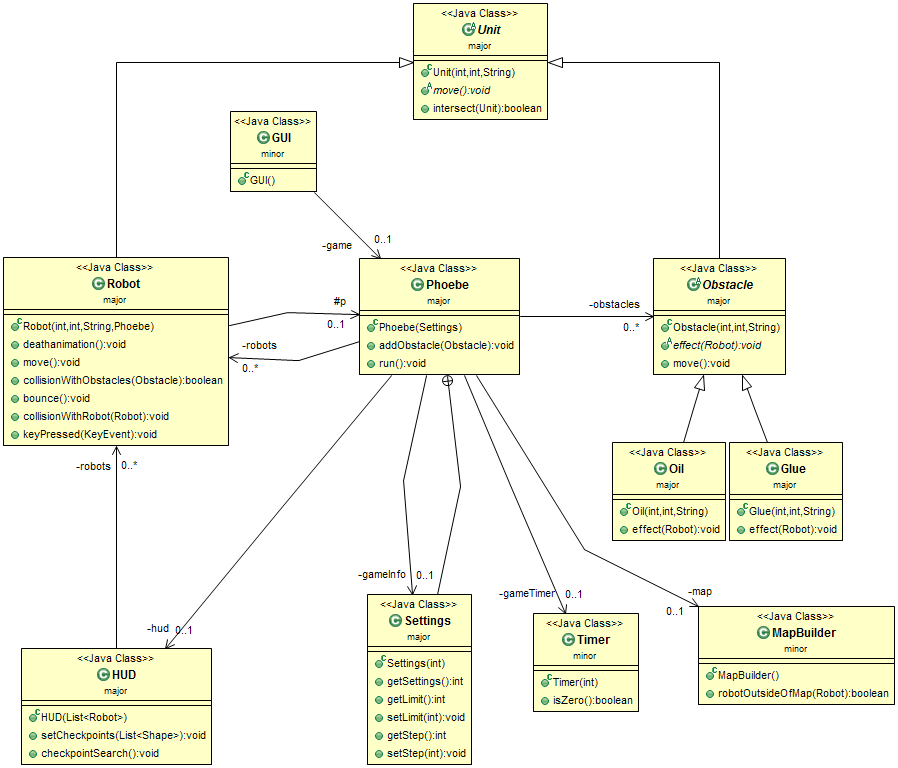
\includegraphics[width=17cm]{images/struktdiagram.PNG}
\caption{Statikus struktúra diagram}
\label{fig:example3}
\end{center}
\end{figure}
\pagebreak
\pagebreak

\section{Szekvencia diagramok}

\subsection{Robot::CheckpointSearch}
\begin{figure}[h]
\begin{center}
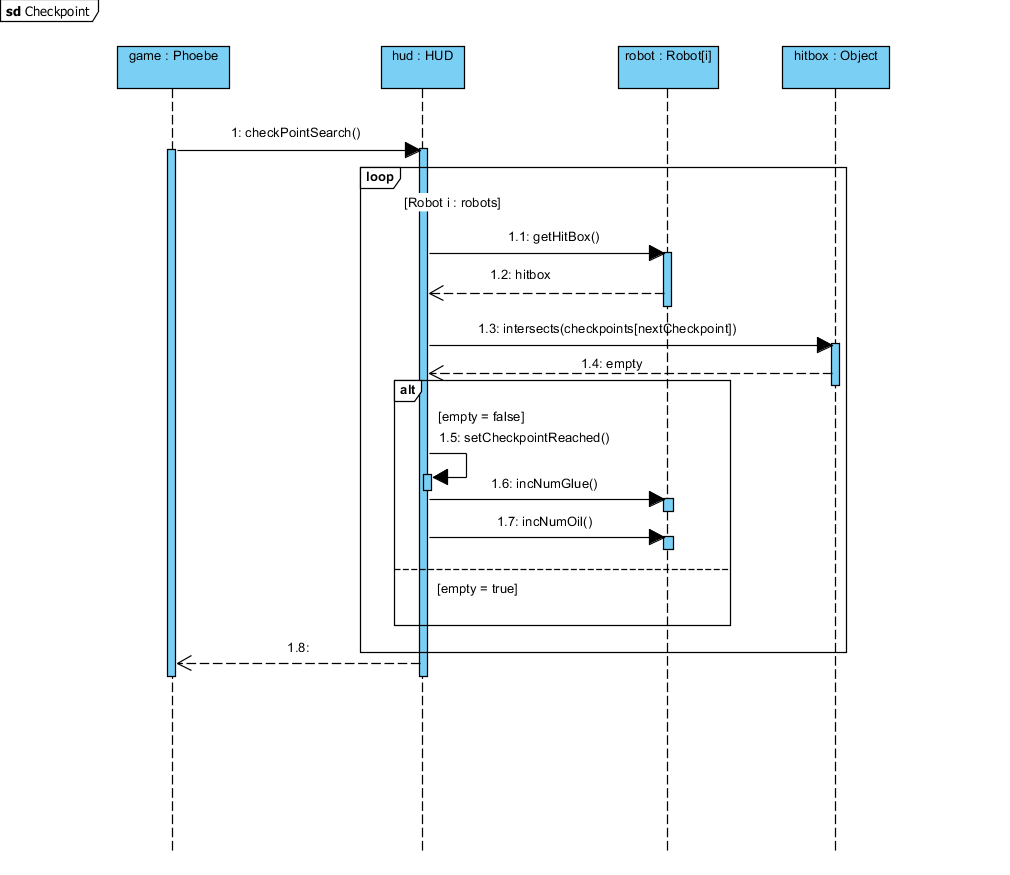
\includegraphics[width=17cm]{images/CheckpointSearch.PNG}
\caption{Következő checkpoint vizsgálata}
\label{fig:example2}
\end{center}
\end{figure}
\pagebreak

\subsection{Robot::CollisonWithObstacle}
\begin{figure}[h]
\begin{center}
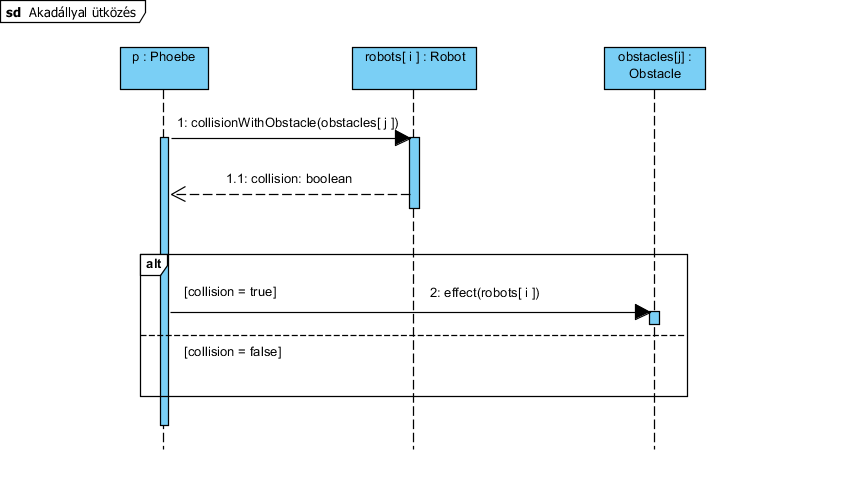
\includegraphics[width=17cm]{images/collisionWithObstacle()_sequence.PNG}
\caption{Robot ütközése akadállyal}
\label{fig:example4}
\end{center}
\end{figure}
\pagebreak

\subsection{Robot::CollisionWithRobot}
\begin{figure}[h]
\begin{center}
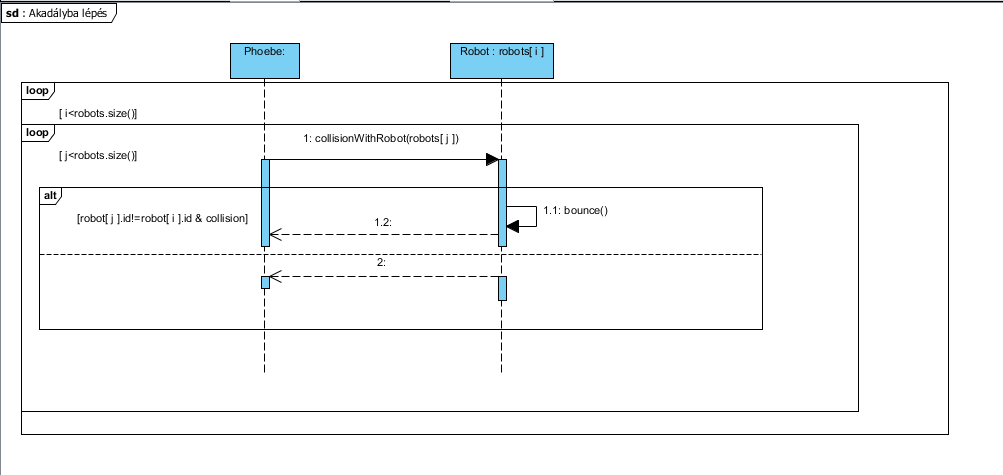
\includegraphics[width=17cm]{images/collisionWithRobot()_sequence.PNG}
\caption{Robot ütközése akadállyal}
\label{fig:example5}
\end{center}
\end{figure}
\pagebreak

\subsection{Robot::FallDown}
\begin{figure}[h]
\begin{center}
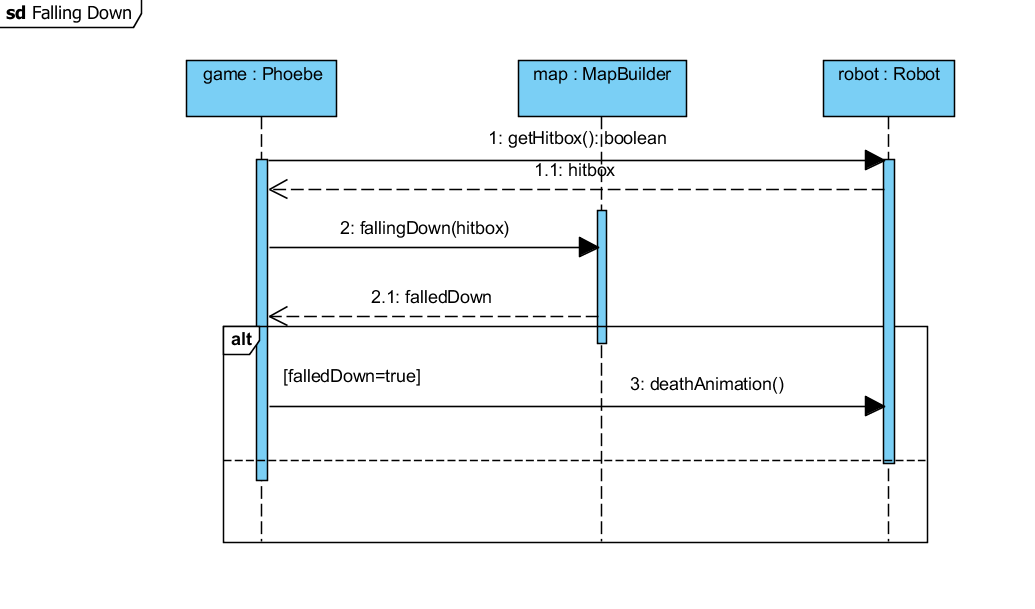
\includegraphics[width=17cm]{images/FallingDown.PNG}
\caption{Robot leesése a pályáról}
\label{fig:example6}
\end{center}
\end{figure}
\pagebreak

\subsection{Robot::InitGame}
\begin{figure}[h]
\begin{center}
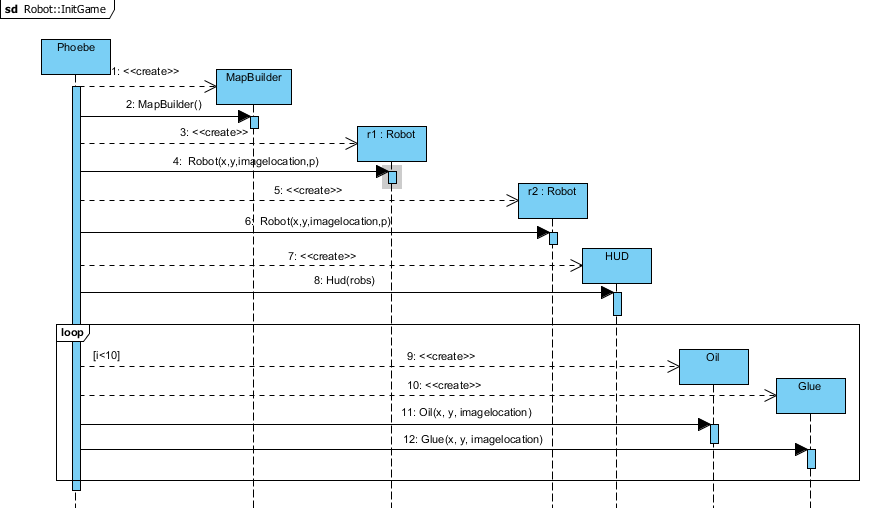
\includegraphics[width=17cm]{images/RobotInitGame.PNG}
\caption{A játék inicializálása}
\label{fig:example7}
\end{center}
\end{figure}
\pagebreak

\subsection{Robot::Move}
\begin{figure}[h]
\begin{center}
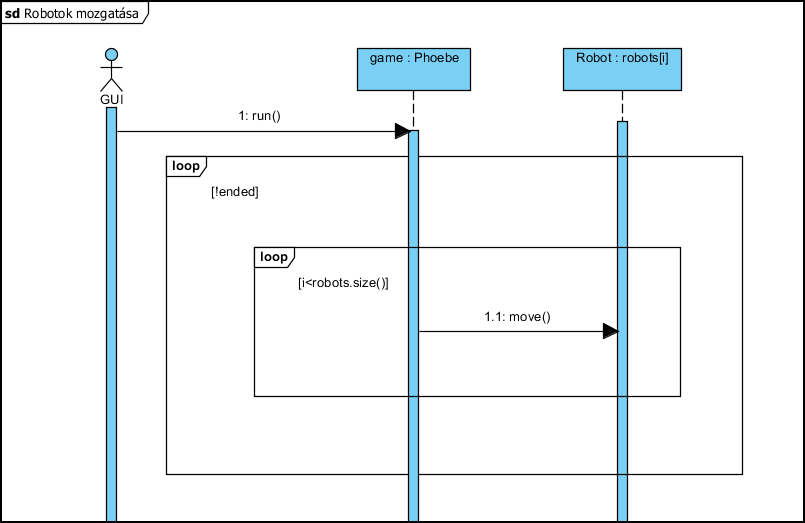
\includegraphics[width=17cm]{images/RobotMove.png}
\caption{A robot mozgatása}
\label{fig:example8}
\end{center}
\end{figure}
\pagebreak

\subsection{Robot::NewObstacle}
\begin{figure}[h]
\begin{center}
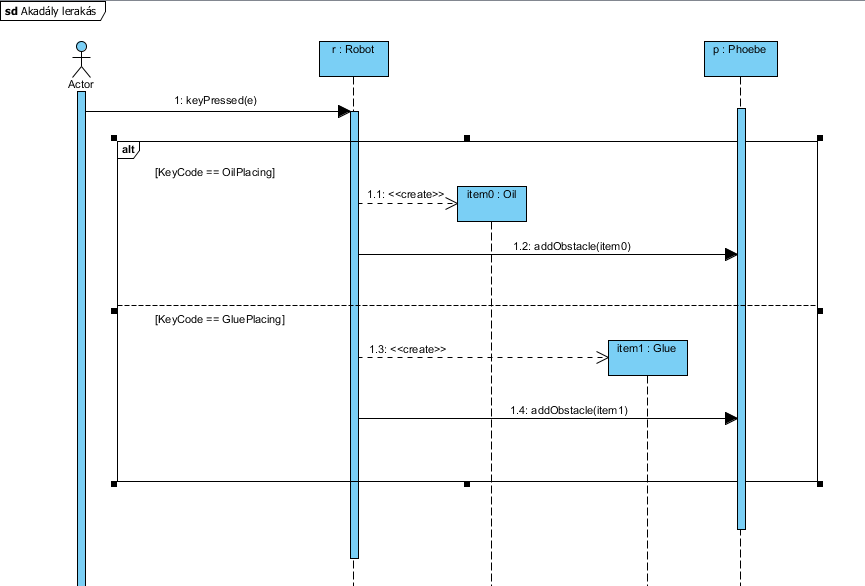
\includegraphics[width=17cm]{images/RobotAddObstacle.png}
\caption{Akadály lerakása}
\label{fig:example9}
\end{center}
\end{figure}
\pagebreak

\subsection{Robot::Settings}
\begin{figure}[h]
\begin{center}
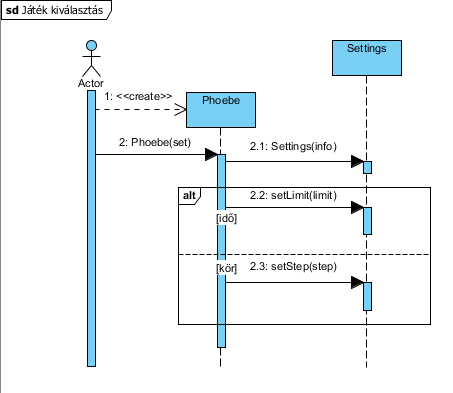
\includegraphics[width=17cm]{images/kivalasztas.PNG}
\caption{A játék beállításainak kiválasztása}
\label{fig:example10}
\end{center}
\end{figure}
\pagebreak

\subsection{Robot::End}
\begin{figure}[h]
\begin{center}
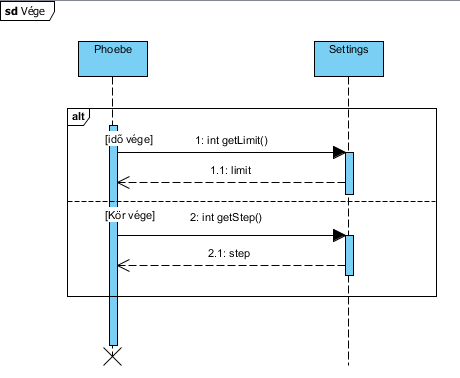
\includegraphics[width=17cm]{images/end.PNG}
\caption{Játék vége}
\label{fig:example11}
\end{center}
\end{figure}
\pagebreak



\section{State-chartok}
\subsection{Robot::States}
\begin{figure}[h]
\begin{center}
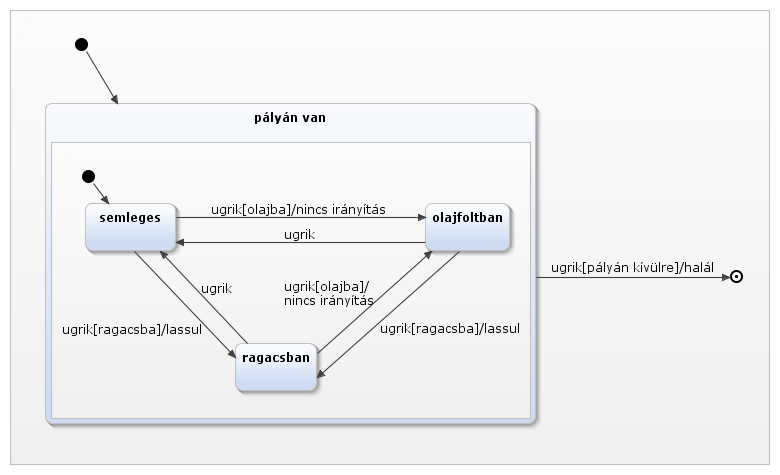
\includegraphics[width=17cm]{images/robot.png}
\caption{A robot állapotai}
\label{fig:example12}
\end{center}
\end{figure}


%% Szglab4
% ===========================================================================
%
\section{Napló}

\begin{naplo}

\bejegyzes
{2010.03.21.~18:00~} % Kezdet
{2,5 óra} % Időtartam
{Horváth\newline
Németh\newline
Tóth\newline
Oláh} % Résztvevők
{Értekezlet. Döntés: Horváth elkészíti az osztálydiagramot, Oláh a use-case leírásokat.} % Leírás

\bejegyzes
{2010.03.23.~23:00~}
{5 óra}
{Németh}
{Tevékenység: Németh implementálja a tesztelő programokat.}

\bejegyzes
{...}
{...}
{...}
{...}


\end{naplo}



%\setcounter{chapter}{3}
%% Szglab4
% ===========================================================================
%
\chapter{Analízis modell kidolgozása 2}

\thispagestyle{fancy}

\section{Objektum katalógus}

\subsection{Glue}
A „Glue” objektum megvalósít egy adott tulajdonságú akadályt. Amely robot belemegy, annak a sebességét megfelezi. 
\subsection{GUI}
A grafikus felületet megvalósító objektum. Ez az objektum maga a menü, ami a játék indítása után ugrik fel. Itt találhatóak a beállítások (mint például a gondolkodás idő és a maximális játék idő vagy a körök száma) és a játékmódok. Gombnyomásra fogja elindítani a játék működési szálát. Ez az objektum kezeli az ablak eseményeit és a játék bezárását.
\subsection{HUD}
Ez az objektum követi és nyilvántartja, hogy a robotok hány checkpoint-on mentek át, mennyi olaj és ragacs van náluk amit felhasználhatnak, illetve kiírja a képernyőre a hátramaradó időt és a megtett körök számát. Feladata, hogy minden körben megvizsgálja, hogy a robotok elérték-e a következő checkpointot.
\subsection{MapBuilder}
Fájlból beolvassa és létrehozza a memóriában a pályát, a kezdő pozíciókat és a checkpointokat reprezentáló objektumokat.  Mivel a  MapBuilder objektum tárolja a pályát így feladat, hogy vizsgálja a robotok azon belül tartózkodását.  
\subsection{Oil}
Ez az objektum az Obstacle osztály leszármazottja. Hasonlóan a Glue objektumhoz, egy adott hatást valósít meg, ami letiltja a következő körben történő irányítását a robotnak, ami belelépett.
\subsection{Phoebe}
A játék logikát megvalósító objektum. Listában tárolja a pályán tartózkodó robotokat, akadályokat és figyeli, hogy mikor ér véget a játék. A „Phoebe” objektum rajzolja ki az objektumokat a pályán és szálként indítható osztályt, melyben maga a játék fut. Játékindításkor berakja a pályára a robotokat és az akadályokat a kezdő pozíciókba. Ebben az objektumban történnek az ellenőrzések (akadályba vagy robotba ütközések, pályáról leesés).
\subsection{Robot}
Olyan objektum, mely a pályán található robotokat valósítja meg. Leírja a viselkedésüket és a kezelésüket. A „Robot” osztály a Unit-ból származik le, ezáltal van pozíciója és az ütközés is le van kezelve. Felelős a mozgásért, megállapítja egy adott akadállyal vagy robottal ütközött-e és kezeli a felhasználó által leütött gombokat.
\subsection{Timer}
Az eltelt időt és a fennmaradt idő nyilvántartásáért felelős. Ilyen például a játék elején a három másodperces visszaszámlálás vagy az időlimites játékmód esetén, amikor a maximális időtől számol visszafelé.

\section{Statikus struktúra diagramok}

\begin{figure}[h]
\begin{center}
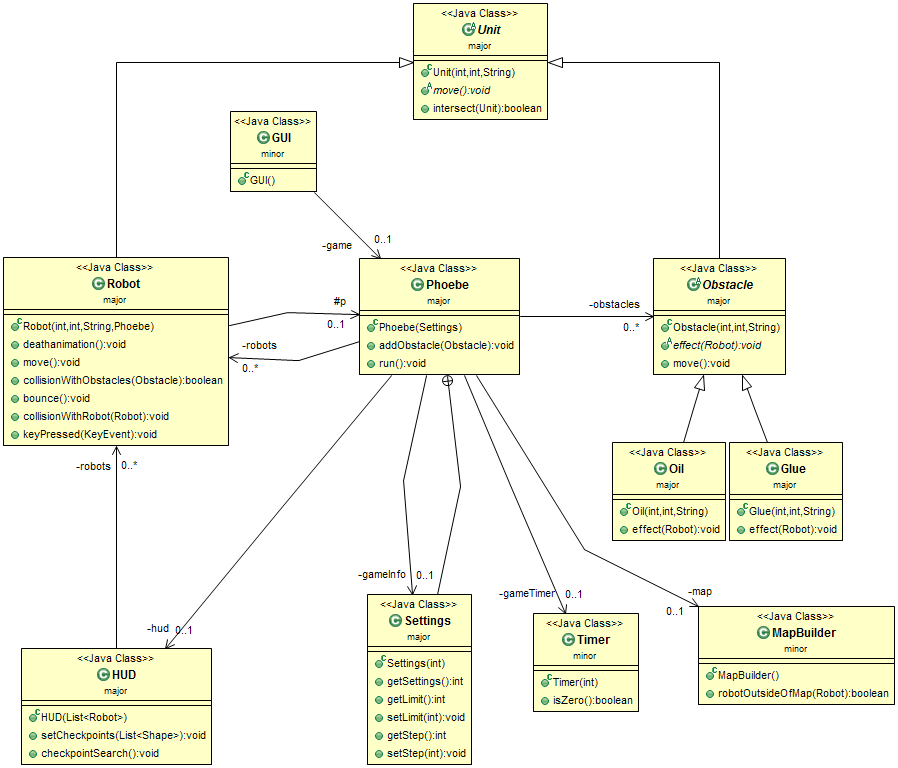
\includegraphics[width=17cm]{images/struktdiagram.PNG}
\caption{Statikus struktúra diagram}
\label{fig:example3}
\end{center}
\end{figure}
\pagebreak
\pagebreak

\begin{figure}[h]
\begin{center}
%\includegraphics[width=17cm]{chapters/chapter04/example.pdf}
\caption{x}
\label{fig:example3}
\end{center}
\end{figure}


\section{Osztályok leírása}
\subsection{Glue}
\begin{itemize}
\item Felelősség\\
A játékban szereplő Ragacs foltok viselkedését leíró osztály
\item Ősosztályok\\
Unit$\rightarrow$Obstacle
\item Metódusok
	\begin{itemize}
		\item void \textbf{effect}(Robot r): Ütközéskor hívja meg az ütközést vizsgáló függvénye a Robot osztálynak. Módosítja a robot slowed értékét 50\%-ra a robot slowed attribútum setterének meghívásával.
	\end{itemize}
\end{itemize}

\subsection{GUI}
\begin{itemize}
\item Felelősség\\
A grafikus felületért felelős osztály, amely a menüt és a játékot jeleníti meg.
\item Attribútumok
	\begin{itemize}
		\item \textbf{Phoebe} game: referencia a játékra
	\end{itemize}
\item Metódusok
	\begin{itemize}
		\item\textbf{GUI}(): Konstruktor. Beállítja az ablak nevét, létrehozza az ablak elemeit, elrendezi őket és beállítja a figyelőket(ActionListener).
	\end{itemize}
\end{itemize}

\subsection{HUD}
\begin{itemize}
\item Felelősség\\
A robotok ragacs- és olajkészletét, illetve megtett köreit és checkpontjait számolja. Megvalósítja a checkpoint ellenőrzést.
\item Attribútumok
	\begin{itemize}
		\item \textbf{int[]} checkpointReached: Minden robothoz külön tárolja a legutoljára érintett checkpoint sorszámát.
		\item \textbf{int[]} lap: Minden robothoz tárolja a megtett körök számát. 
		\item \textbf{int[]} numGlue: Minden robothoz tárolja a ragacsok számát.
		\item \textbf{int[]} numOil: Minden robothoz tárolja az olajok számát.
		\item \textbf{List<Shape>} checkpoints: Tárolja a checkpointokat reprezentáló objektumokat List adatszerkezetben. A checkpointSearch függvény kérdezi le ebből a következő checkpoint helyzetét. 
		\item \textbf{List<Robot>} robots: A robotokat tároló List adatszerkezet. A checkpointSearch függvény kérdezi le ebből a robotokat, majd azok helyzetét.
	\end{itemize}
\item Metódusok
	\begin{itemize}
		\item \textbf{HUD}(List<Robot> robs): Konstruktor, inicializálja a köröket számláló változót, az érintett checkpointokat, a ragacs és olajkészleteket. 
		\item void \textbf{checkpointSearch}(): Ellenőrzi hogy a robotok teljesítették-e a következő checkpointot.
		\item void \textbf{setCheckpoints}(List<Shape> checkObj): Checkpointokat reprezentáló adatszerkezet betöltése.
		
	\end{itemize}
\end{itemize}

\subsection{MapBuilder}
\begin{itemize}
\item Felelősség\\
A pálya felépítéséért, a checkpointok tárolásáért és a robot pályán tartózkodásának vizsgálatáért felelős osztály.
\item Attribútumok
	\begin{itemize}
		\item \textbf{Shape} map: A pályát reprezentáló objektum. 
		\item \textbf{List<Shape>} checkpoints: Tárolja a checkpointokat reprezentáló objektumokat List adatszerkezetben.
		\item \textbf{int[]} startPosPlayerOne: Meghatároz egy (x,y) koordinátát, ahol az első játékos kezd.
		\item \textbf{int[]} startPosPlayerTwo: Meghatároz egy (x,y) koordinátát, ahol az második játékos kezd.
	\end{itemize}
\item Metódusok
	\begin{itemize}
		\item \textbf{MapBuilder}(): Konstruktor, a pálya beolvasása fájlból, majd létrehozása.
		\item boolean \textbf{fallingDown}(Shape othershape): Igaz értéket ad vissza, ha a robot leesett a pályáról, hamisat ha még rajta van.
	\end{itemize}
\end{itemize}

\subsection{Obstacle}
\begin{itemize}
\item Felelősség\\
A pályán/játékosoknál lévő különböző akadályokat (ragacs,olaj) összefogó ősosztály.
\item Ősosztályok\\
Unit
\item Attribútumok
	\begin{itemize}
		\item \textbf{int} WIDTH: Az akadályokat jellemző szélesség. Szükség van rá, hogy létrehozzuk a leszármazottak hitbox-át(sokszög pályaelem).
		\item \textbf{int} HEIGHT: Az akadályokat jellemző hosszúság. Szükség van rá, hogy létrehozzuk a leszármazottak hitbox-át(sokszög pályaelem).
	\end{itemize}
\item Metódusok
	\begin{itemize}
		\item \textbf{Obstacle}(int x, int y, String imagelocation): meghívja a Unit konstruktorát a megadott adatokkal és létrehoz egy sokszög elemet ami reprezentálja a pályán majd.
		\item void \textbf{effect}(Robot r): Meghatározza, milyen hatással van a robotra, ha érintkezik egy Obstacle-lel. Absztrakt.
	\end{itemize}
\end{itemize}

\subsection{Oil}
\begin{itemize}
\item Felelősség\\
A pályára lerakható olaj megvalósítása. Ha belelép egy játékos egy ilyen olajfoltba, az effect függvény letiltja a mozgatást az adott roboton a következő ugrásig.
\item Ősosztályok\\
Unit $\rightarrow$ Obstacle 
\item Metódusok
	\begin{itemize}
		\item \textbf{Oil}(int x, int y, String imagelocation): Egy Oil elem létrehozásáért felelős.
		\item void \textbf{effect}(Robot r): Meghatározza, milyen hatással van a robotra, ha beleugrik egy olajfoltba. Ebben az esetben letiltja a játékost, hogy irányt váltson.
	\end{itemize}
\end{itemize}

\subsection{Phoebe}
\begin{itemize}
\item Felelősség\\
A játék motorját képviselő osztály. A robotok pozíciójáért, az akadályok elhelyezéséért és a játék végéért felel.
\item Attribútumok
	\begin{itemize}
		\item \textbf{boolean} ended: Állapot változó, ha vége a játéknak, akkor true. Ha beteljesül egy játék végét jelentő esemény, akkor ezen a változón keresztül leáll a játék és megállapítódik a nyertes.
		\item \textbf{List<Robot>} robots: A játékban szereplő robotok listája.
		\item \textbf{List<Obstacle>} obstacles: A játékban szereplő akadályok listája.
		\item \textbf{HUD} hud: A játékosok előrehaladását, ragacs és olajkészleteit tartja számon
		\item \textbf{MapBuilder} map: 
	\end{itemize}
\item Metódusok
	\begin{itemize}
		\item \textbf{Phoebe}(Setting set): A játék felépítése, a robotok lista, az akadályok lista létrehozása
		\item void \textbf{run}(): Ez a metódus futtatja a főciklust, amelyben maga a játék működik.
	\end{itemize}
\end{itemize}

\subsection{Robot}
\begin{itemize}
\item Felelősség\\
A játékban résztvevő robotok viselkedését és kezelését leíró osztály.
\item Ősosztályok\\
Unit
\item Interfészek\\
Nincs interfésze
\item Attribútumok
	\begin{itemize}
		\item \textbf{int} staticID: Az osztályhoz tartozó statikus azonosító, a példány                azonosítójának(id) meghatározásához szükséges.
		\item \textbf{int} HEIGHT: A robot képének magassága, collision                      detektálásnál, továbbá az irányítást segítő nyíl kezdő koordinátájának                  meghatározásánál szükséges.
		\item \textbf{int} WIDTH: A robot képének szélessége, funkcionalitásban hasonló a WIDTH-hez.
		\item \textbf{int} ID: A robot példányának egyedi azonosítója, a keyconfig sorának                     indexelésére szükséges.
		\item \textbf{double} slowed: A sebesség módosításáért felel, default értéke 1.0. Amennyiben ragacsba lép a robot ez 0.5-re módosul és minden ugrás végén visszaáll az eredeti értékére. Ugrásnál ezzel szorozzuk be a végkordinátát kiszámító sugár hosszát.
		\item \textbf{boolean} oiled: Azt jelzi, hogy olajba lépett-e. Ennek hatására a mozgás iránya módosíthatatlanná válik egy kis időre. 
		\item \textbf{int} arrowendx: A robot irányítását segítő nyílnak az x koordinátája, a nyíl kirajzolásánál van szerepe.
		\item \textbf{int} arrowendy: A robot irányítását segítő nyílnak az y koordinátája, a nyíl kirajzolásánál van szerepe.
		\item \textbf{double} alpha: A robot irányítását segítő nyíl vízszintessel bezárt szöge. A nyil kirajzolásánál, az ugrás végpontjának meghatározánál van szerepe.
		\item \textbf{boolean} moved: Azt jelöli, hogy lépett-e már a robot az aktuális körben. A megjelenítésnél (a nyilat ugrás közben nem jelenítjük meg), illetve az irányítás letiltásánál van szerepe (olajba lépés esetén).
		\item \textbf{int[][]} keyconfig: A játékosok írányítását tároló mátrix. A játékosok irányítását ennek segítségével határozzuk meg a keyPressed függvényben. A sor meghatározza a felhasználóhoz tartozó gombokat, az oszlopok a funkciók (olaj/ragacs lerakás, a nyíl jobbra/balra mozgatása).
\end{itemize}
\item Metódusok\\
	\begin{itemize}
		\item \textbf{Robot}(int x,int y,String imagelocation,Phoebe p): Létrehoz egy robotot a megadott x,y koordinátákon, betölti a képét az imagelocation cím alapján, továbbá eltárolja a játékmotor referenciáját.
		\item \textbf{void deathanimation}(): A Robot halálának grafikus megjelenítéséért felelős függvény.
		\item boolean \textbf{collisionWithObstacle}(Obstacle o): Ellenőrzi hogy a robot ütközött-e az akadállyal. Igazzal tér vissza ha igen, hamissal ha nem.
		\item void \textbf{collisionWithRobot}(Robot r): Ellenőrzi, hogy a robot ütközött-e másik robottal. Ha igen, akkor gondoskodik róla, hogy a robotok a megfelelő szögben pattanjanak le egymásról.
		\item void \textbf{keyPressed}(Keyevent e): A robot irányítását megvalósító függvény, a játékmotor keylistener-e által hívódik meg, a lenyomott billentyű keyevent-jére. A következő ugrás beállítása, a ragacs/olaj lerakása történhet itt a keyconfig változó felhasználásával.
	\end{itemize}
\end{itemize}

\subsection{Timer}
\begin{itemize}
\item Felelősség\\
A visszaszámlálásért (idő, director time) felelős.
\item Metódusok
	\begin{itemize}
		\item \textbf{Timer}(int i): Konstruktor; inicializál egy viszaszámláló órát.
		\item boolean \textbf{isZero}(): Igazzal tér vissza, ha a megadott idő lejárt.
	\end{itemize}
\end{itemize}

\subsection{Unit}
\begin{itemize}
\item Felelősség\\
A pályán található objektumokért felel és azok viszonyáról (például ütközésükről).
\item Attribútumok
	\begin{itemize}
		\item \textbf{int} x: Az egység x koordinátája
		\item \textbf{int} y: Az egység y koordinátája
		\item \textbf{Rectangle} hitbox: Az egységet a pályán reprezentáló sokszög.
	\end{itemize}
\item Metódusok
	\begin{itemize}
		\item void \textbf{move}() : Absztrakt függvény, mely a leszármazottakban fog megvalósulni. Az egységek mozgásáért felelős.
		\item boolean \textbf{intersect}(Unit u): Két egység ütközését meghatározó függvény.
	\end{itemize}
\end{itemize}
\pagebreak

\section{Szekvencia diagramok}

\subsection{Robot::CheckpointSearch}
\begin{figure}[h]
\begin{center}
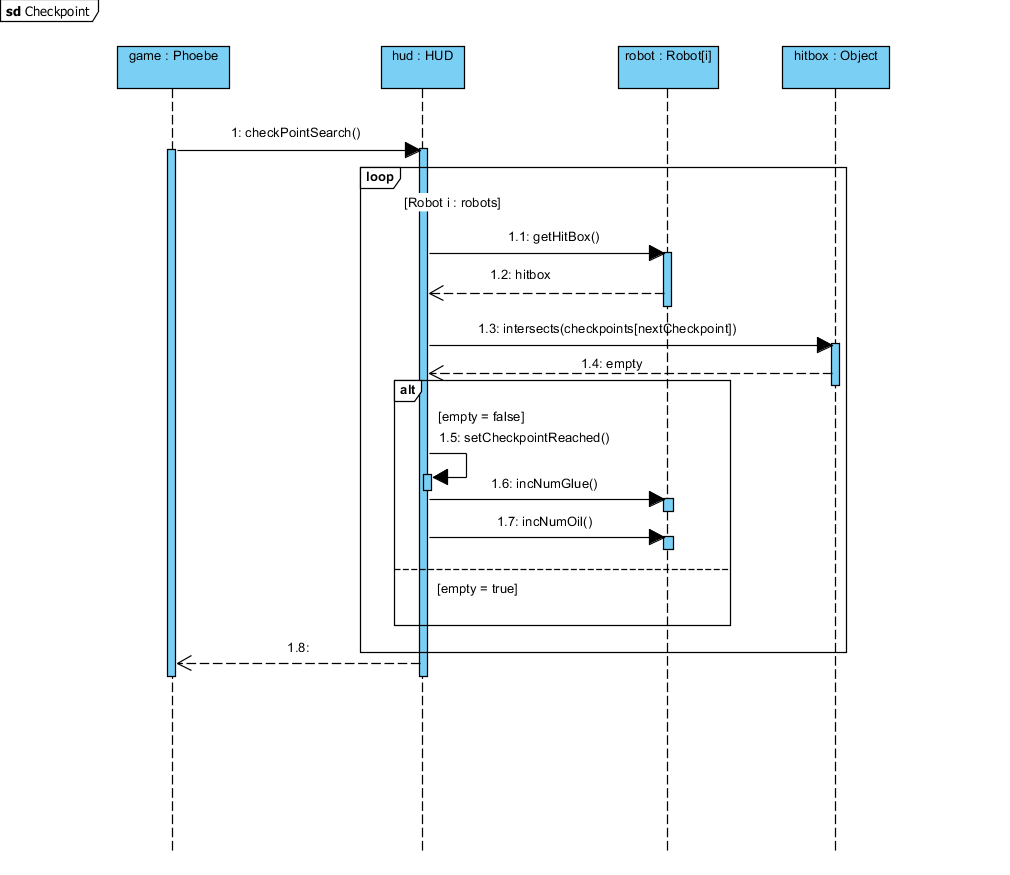
\includegraphics[width=17cm]{images/CheckpointSearch.PNG}
\caption{Következő checkpoint vizsgálata}
\label{fig:example2}
\end{center}
\end{figure}
\pagebreak

\subsection{Robot::CollisonWithObstacle}
\begin{figure}[h]
\begin{center}
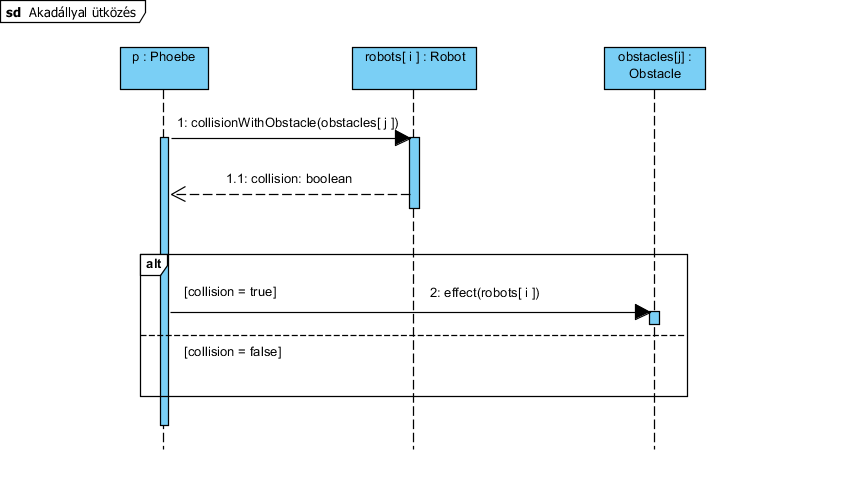
\includegraphics[width=17cm]{images/collisionWithObstacle()_sequence.PNG}
\caption{Robot ütközése akadállyal}
\label{fig:example4}
\end{center}
\end{figure}
\pagebreak

\subsection{Robot::CollisionWithRobot}
\begin{figure}[h]
\begin{center}
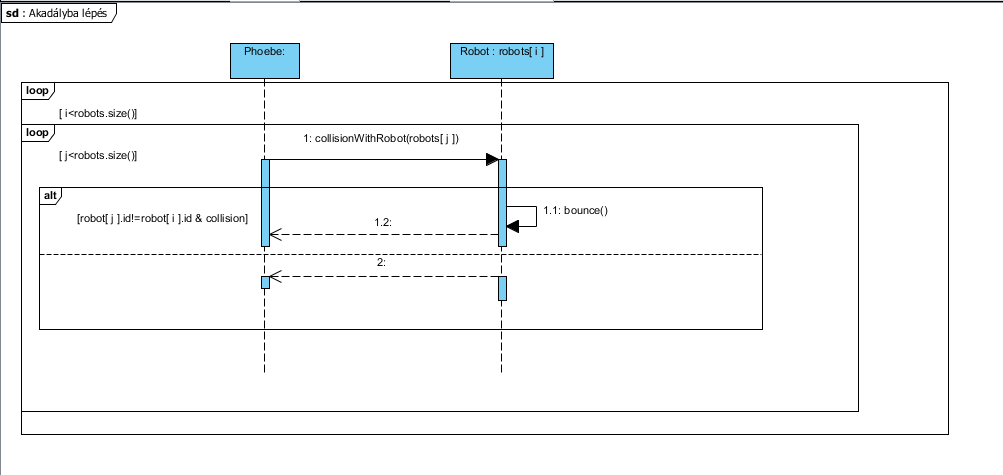
\includegraphics[width=17cm]{images/collisionWithRobot()_sequence.PNG}
\caption{Robot ütközése másik robottal}
\label{fig:example5}
\end{center}
\end{figure}
\pagebreak

\subsection{Robot::FallDown}
\begin{figure}[h]
\begin{center}
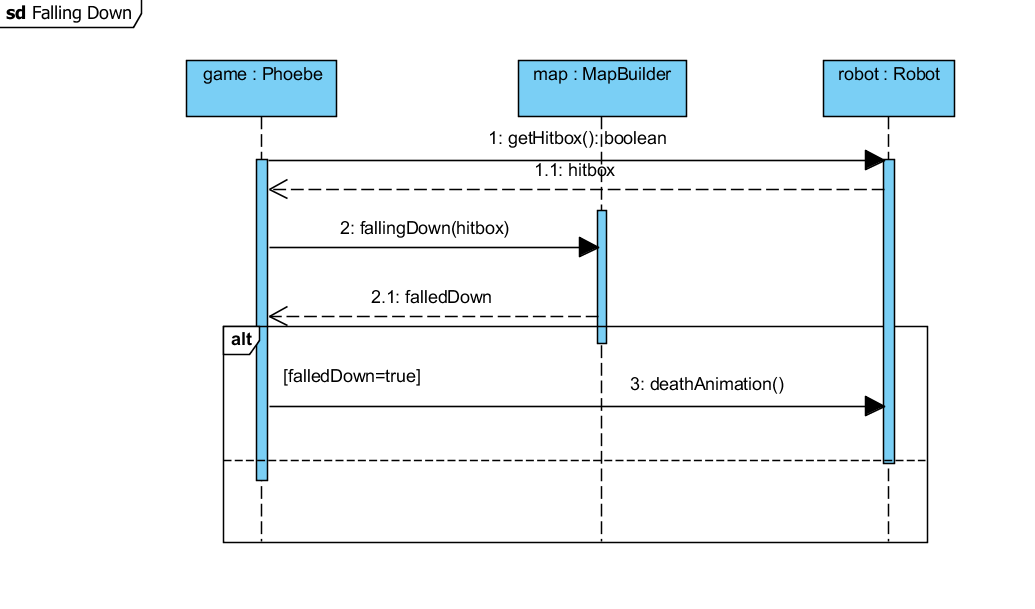
\includegraphics[width=17cm]{images/FallingDown.PNG}
\caption{Robot leesése a pályáról}
\label{fig:example6}
\end{center}
\end{figure}
\pagebreak

\subsection{Robot::InitGame}
\begin{figure}[h]
\begin{center}
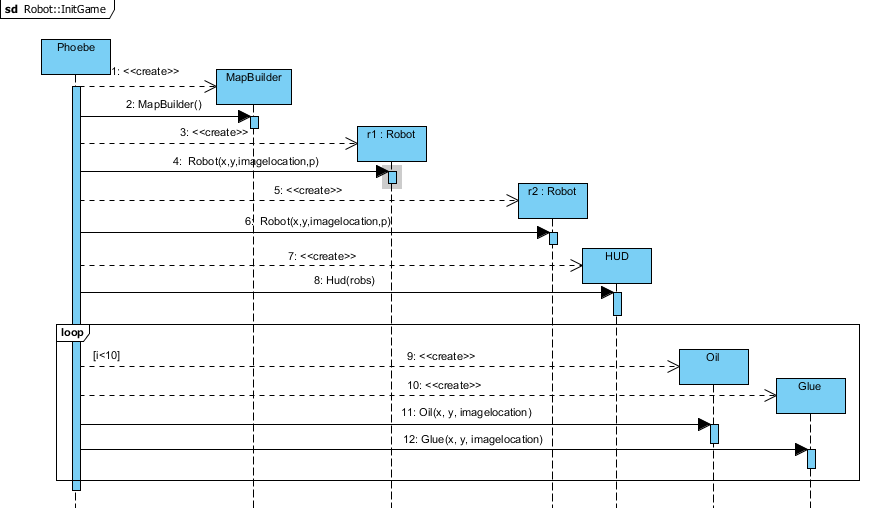
\includegraphics[width=17cm]{images/RobotInitGame.PNG}
\caption{A játék inicializálása}
\label{fig:example7}
\end{center}
\end{figure}
\pagebreak

\subsection{Robot::Move}
\begin{figure}[h]
\begin{center}
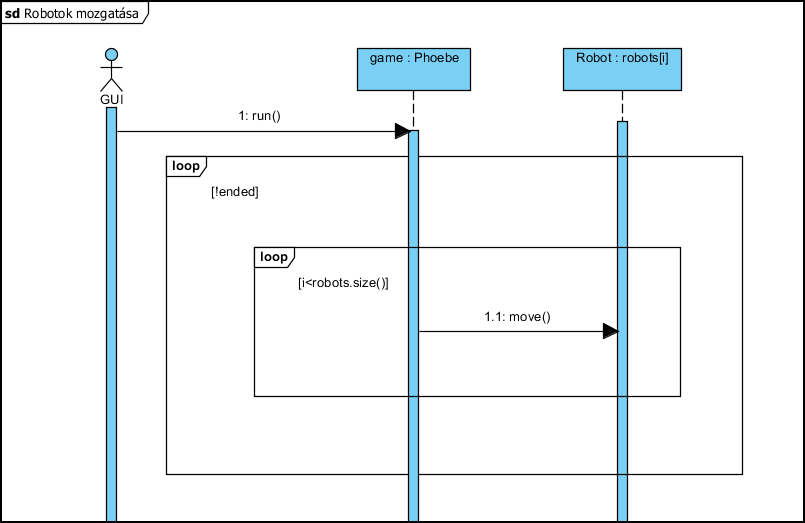
\includegraphics[width=17cm]{images/RobotMove.png}
\caption{A robot mozgatása}
\label{fig:example8}
\end{center}
\end{figure}
\pagebreak

\subsection{Robot::NewObstacle}
\begin{figure}[h]
\begin{center}
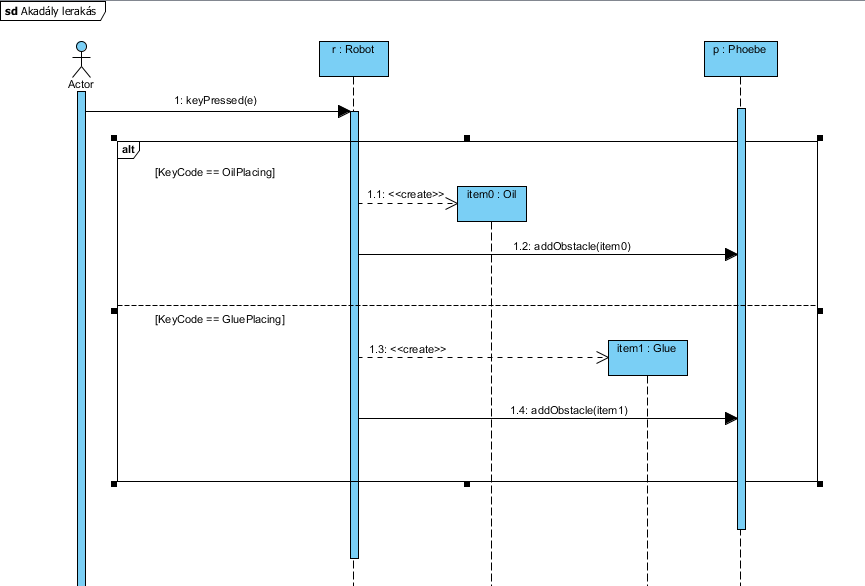
\includegraphics[width=17cm]{images/RobotAddObstacle.png}
\caption{Akadály lerakása}
\label{fig:example9}
\end{center}
\end{figure}
\pagebreak

\subsection{Robot::Settings}
\begin{figure}[h]
\begin{center}
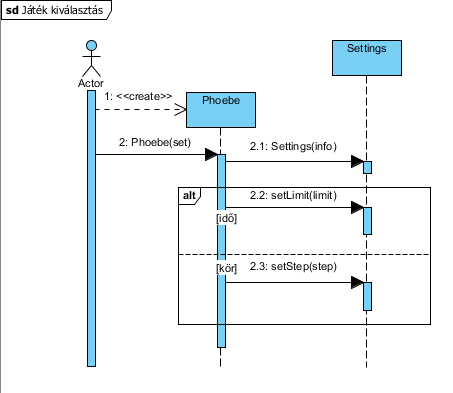
\includegraphics[width=17cm]{images/kivalasztas.PNG}
\caption{A játék beállításainak kiválasztása}
\label{fig:example10}
\end{center}
\end{figure}
\pagebreak

\subsection{Robot::End}
\begin{figure}[h]
\begin{center}
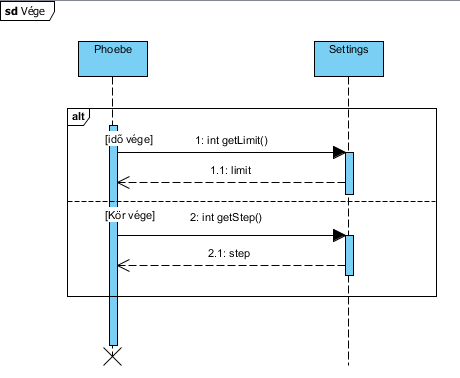
\includegraphics[width=17cm]{images/end.PNG}
\caption{Játék vége}
\label{fig:example11}
\end{center}
\end{figure}
\pagebreak

\section{State-chartok}

\subsection{Robot::States}
\begin{figure}[h]
\begin{center}
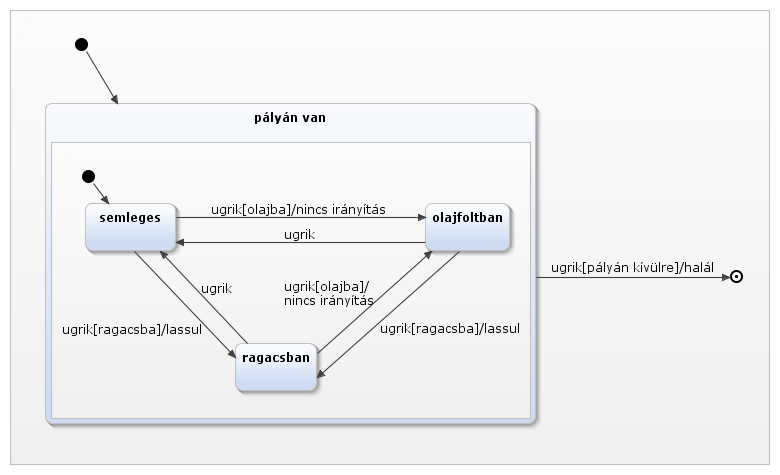
\includegraphics[width=17cm]{images/robot.png}
\caption{A robot állapotai}
\label{fig:example12}
\end{center}
\end{figure}
%% Szglab4
% ===========================================================================
%
\pagebreak
\section{Napló}

\begin{naplo}

\bejegyzes
{2015.03.04.~8:15~} % Kezdet
{2 óra} % Időtartam
{Kovács\newline
Lovász\newline
Tóth\newline
Graics\newline
Magyar
} % Résztvevők
{Konzultáció, részfeladatok kiosztása}

\bejegyzes
{2015.03.06.~17:00~}
{3 óra}
{Magyar\newline
Tóth}
{Analízis modell finomítása, hibáinak kijavítása}


\end{naplo}



%\setcounter{chapter}{4}
%% Szglab4
% ===========================================================================
%
\chapter{Szkeleton tervezése}

\thispagestyle{fancy}

\section{A szkeleton modell valóságos use-case-ei}
\comment{A szkeletonnak, mint önálló programnak a működésével kapcsolatos use-case-ek.}

\subsection{Use-case diagram}

\begin{figure}[h]
\begin{center}
%\includegraphics[width=17cm]{chapters/chapter05/example.pdf}
\caption{x}
\label{fig:SzkeletonUseCase}
\end{center}
\end{figure}

\subsection{Use-case leírások}
\comment{Minden use-case-hez külön}

\usecase{...}{...}{...}{...}

\section{A szkeleton kezelői felületének terve, dialógusok}
\comment{A szkeleton által elfogadott bemenetek , valamint a szöveges konzolon megjelenő kimenetek. A kiemenet formátuma olyan kell legyen, ami alapján a működés összevethető a korábbi szekvencia-diagramokkal.}

\section{Szekvencia diagramok a belső működésre}
\comment{A szkeletonban implementált szekvenciadiagramok. Tipikusan egy use-case egy diagram. Ezek megegyezhetnek a korábban specifikált diagramokkal, de az egyes életvonalakat (lifeline) egyértelműen a szkeletonban példányosított objektumokhoz kell tudni kötni. Azt kell megjeleníteni, hogy a szkeletonban létrehozott objektumok egymással hogyan fognak kommunikálni.}

\section{Kommunikációs diagramok}
\comment{A szkeletonban, az egyes szkeleton-use-case-ek futása során létrehozott objektumok és kapcsolataik bemutatására szolgáló diagramok. Ezek alapján valósítják meg a szkeleton fejlesztői az inicializáló kódrészleteket.}

%% Szglab4
% ===========================================================================
%
\pagebreak
\section{Napló}

\begin{naplo}

\bejegyzes
{2015.03.04.~11:00~}
{5 óra}
{Kovács}
{Szkeleton tervezés}

\bejegyzes
{2015.03.05.~9:00~}
{1,5 óra}
{Lovász}
{Use-case diagramm készítés}

\bejegyzes
{2015.03.09.~16:15~} % Kezdet
{2,5 óra} % Időtartam
{Kovács\newline
Lovász\newline
Tóth\newline
Graics\newline
Magyar
} % Résztvevők
{Konzultáció, részfeladatok kiosztása}


\end{naplo}


%
\setcounter{chapter}{5}
% Szglab4
% ===========================================================================
%
\chapter{Szkeleton beadás}

\thispagestyle{fancy}

\section{Fordítási és futtatási útmutató}
\comment{A feltöltött program fordításával és futtatásával kapcsolatos útmutatás. Ennek tartalmaznia kell leltárszerűen az egyes fájlok pontos nevét, méretét byte-ban, keletkezési idejét, valamint azt, hogy a fájlban mi került megvalósításra.}

\subsection{Fájllista}

\begin{fajllista}

\fajl
{Main.java} % Kezdet
{250 byte} % Idptartam
{2009.10.10~18:05~} % Résztvevők
{...} % Leírás

\fajl
{...}
{...}
{...}
{...}

\end{fajllista}

\subsection{Fordítás}
\comment{A fenti listában szereplő forrásfájlokból milyen műveletekkel lehet a bináris, futtatható kódot előállítani. Az előállításhoz csak a 2. Követelmények c. dokumentumban leírt környezetet szabad előírni.}

\lstset{escapeinside=`', xleftmargin=10pt, frame=single, basicstyle=\ttfamily\footnotesize, language=sh}
\begin{lstlisting}
javac -d bin *.java
\end{lstlisting}

\subsection{Futtatás}
\comment{A futtatható kód elindításával kapcsolatos teendők leírása. Az indításhoz csak a 2. Követelmények c. dokumentumban leírt környezetet szabad előírni.}

\lstset{escapeinside=`', xleftmargin=10pt, frame=single, basicstyle=\ttfamily\footnotesize, language=sh}
\begin{lstlisting}
cd bin
java Main.java
\end{lstlisting}

\section{Értékelés}
\comment{A projekt kezdete óta az értékelésig eltelt időben tagokra bontva, százalékban.}

\begin{ertekeles}
\tag{Horváth} % Tag neve
{23.5}        % Munka szazalekban
\tag{Német}
{24.5}
\tag{Tóth}
{25}
\tag{Oláh}
{27}
\end{ertekeles}


% Szglab4
% ===========================================================================
%
\pagebreak
\section{Napló}

\begin{naplo}

\bejegyzes
{2015.03.18.~8:15~} % Kezdet
{2,5 óra} % Időtartam
{Kovács\newline
Lovász\newline
Tóth\newline
Graics\newline
Magyar
} % Résztvevők
{Konzultáció, részfeladatok kiosztása}

\bejegyzes
{2010.03.20.~18:00~}
{3 óra}
{Kovács}
{Szkeleton use-case implementálása}

\bejegyzes
{2010.03.20.~18:00~}
{3 óra}
{Lovász}
{Szkeleton use-case implementálása}

\bejegyzes
{2010.03.20.~18:00~}
{3 óra}
{Tóth}
{Szkeleton use-case implementálása}

\bejegyzes
{2010.03.20.~18:00~}
{3 óra}
{Graics}
{Szkeleton use-case implementálása}

\bejegyzes
{2010.03.20.~18:00~}
{3 óra}
{Magyar}
{Szkeleton use-case implementálása}

\end{naplo}


%
%\setcounter{chapter}{6}
%%\textit{% Szglab4
% ===========================================================================
%
\setcounter{chapter}{-1}
\chapter{Módosítások}
\comment{Feladatok: Objektum katalógus szövegeinek ellenőrzése, Osztályok leírásának pontjainak ellenőrzése, újonnan hozzáadott elemeinek felelősségének leírása}
\section{Objektum katalógus}
\subsection{HUD}
Ez az objektum követi és nyilvántartja, hogy a robotok hány checkpoint-on mentek át, illetve kiírja a képernyőre a hátramaradó időt és a megtett körök számát. Feladata, hogy minden körben megvizsgálja, hogy a robotok elérték-e a következő checkpointot.
\subsection{MyListener}
\comment{...}

\section{Osztályok leírása}
\subsection{HUD}
\begin{itemize}
\item Felelősség\\
A robotok megtett köreit és checkpontjait tartja számon. Megvalósítja a checkpoint ellenőrzést.
\item Attribútumok
	\begin{itemize}
		\item \textbf{int[]} checkpointReached: Minden robothoz külön tárolja a legutoljára érintett checkpoint sorszámát.
		\item \textbf{int[]} lap: Minden robothoz tárolja a megtett körök számát. 
		\item \textbf{List} checkpoints: Tárolja a checkpointokat reprezentáló objektumokat List adatszerkezetben. A checkpointSearch függvény kérdezi le ebből a következő checkpoint helyzetét. 
		\item \textbf{List<Robot>} robots: A robotokat tároló List adatszerkezet. A checkpointSearch függvény kérdezi le ebből a robotokat, majd azok helyzetét.
	\end{itemize}
\item Metódusok
	\begin{itemize}
		\item \textbf{HUD}(List<Robot> robs): Robot objektumokat tároló ArrayList. Célja, hogy a checkpointsearch() függvényben minden robotra elvégezzük a keresést.
		\item void \textbf{checkpointSearch}(): Minden híváskor ellenőrzi, hogy a robot és a checkpoint metszete üres-e. 
		\item void \textbf{setCheckpoints}(List checkObj): Checkpointokat reprezentáló adatszerkezet betöltése.CheckpointReached inicializálása a checkpointok számától függően.
		\item void \textbf{setCheckpointReached}(Robot r): Ha a paraméterként átadott robot következő checkpointja a célvonal (utolsó checkpoint) akkor lenullázza a checkpointReached-et és növeli a megtett körök számát, illetve ha nem akkor növeli az érintett checkpointok számát.
		\item int \textbf{endOfTheGame}(): A játék végén eldönti, hogy melyik játékos nyert. Visszatér egy számmal, amiből egyértelműen eldönthető, hogy ki nyert. Ha negatív akkor az 1-es számú játékos nyert, ha nulla akkor döntetlen, ha pozitív akkor a 2-es számú játékos nyert.
	\end{itemize}
\end{itemize}

\subsection{IVisible}
\begin{itemize}
\item Felelősség\\
A grafikus motorhoz szükséges interfész. Olyan osztályok, melyek kirajzolható elemeket tartalmaznak megvalósítják ezt az interfészt.
\item Metódusok\\
	\begin{itemize}
		\item void \textbf{paint}(Graphics2D g): Rajzolást elvégző metódus.
	\end{itemize}
\end{itemize}

\subsection{MapBuilder}
\begin{itemize}
\item Felelősség\\
A pálya felépítéséért, a checkpointok tárolásáért és a robot pályán tartózkodásának vizsgálatáért felelős osztály.
\item Attribútumok
	\begin{itemize}
		\item \textbf{List} checkpoints: Tárolja a checkpointokat reprezentáló objektumokat List adatszerkezetben.
		\item \textbf{int[]} startPosPlayerOne: Meghatároz egy (x,y) koordinátát, ahol az első játékos kezd.
		\item \textbf{int[]} startPosPlayerTwo: Meghatároz egy (x,y) koordinátát, ahol az második játékos kezd.
		\item \textbf{Object} map: \comment{...}
	\end{itemize}
\item Metódusok
	\begin{itemize}
		\item \textbf{MapBuilder}(): Konstruktor, a pálya beolvasása fájlból, majd létrehozása.
		\item boolean \textbf{robotOutsideOfMap}(Robot r): Igaz értéket ad vissza, ha a robot leesett a pályáról, hamisat ha még rajta van.
	    \item boolean \textbf{obstacleOutsideOfMap}(Obstacle obs): \comment{...}
	    \item int[] \textbf{getStartPosPlayer}(int id): \comment{...}
	\end{itemize}
\end{itemize}

\subsection{MyListener}
\begin{itemize}
\item Felelősség\\
Nyilvántartja a gombok lenyomását és felengedését. Meghívja a gombhoz tartozó robotnak a gombnyomást lekezelő metódusát.
\item Interfészek\\
KeyListener, Runnable
\item Attribútumok\\
	\begin{itemize}
	    \item \textbf{List} robots: \comment{...}
		\item \textbf{boolean} isUp: \comment{...}
		\item \textbf{boolean} isDown: \comment{...}
		\item \textbf{boolean} isRight: \comment{...}
		\item \textbf{boolean} isLeft: \comment{...}
		\item \textbf{boolean} isW: \comment{...}
		\item \textbf{boolean} isD: \comment{...}
		\item \textbf{boolean} isS: \comment{...}
		\item \textbf{boolean} isA: \comment{...}
	\end{itemize}
\item Metódusok\\
	\begin{itemize}
		\item \textbf{MyListener}(List robots): \comment{...}
		\item void \textbf{run}():  \comment{...}
		\item void \textbf{keyPressed}(KeyEvent e): \comment{...}
		\item void \textbf{keyTyped}(KeyEvent e): \comment{...}
	\end{itemize}
\end{itemize}

\subsection{Obstacle}
\begin{itemize}
\item Felelősség\\
A pályán/játékosoknál lévő különböző akadályokat (ragacs,olaj) összefogó ősosztály.
\item Ősosztályok\\
Unit
\item Attribútumok
	\begin{itemize}
		\item \textbf{int} WIDTH: Az akadályokat jellemző szélesség. Szükség van rá, hogy létrehozzuk a leszármazottak hitbox-át(sokszög pályaelem).
		\item \textbf{int} HEIGHT: Az akadályokat jellemző hosszúság. Szükség van rá, hogy létrehozzuk a leszármazottak hitbox-át(sokszög pályaelem).
		\item \textbf{int} lifetime: Megmondja, hogy hány kör óta lett letéve az akadály.
	\end{itemize}
\item Metódusok
	\begin{itemize}
		\item \textbf{Obstacle}(int x, int y, String imagelocation): Meghívja a Unit konstruktorát a megadott adatokkal és létrehoz egy sokszög elemet ami reprezentálja a pályán majd.
		\item void \textbf{effect}(Robot r): Meghatározza, milyen hatással van a robotra, ha érintkezik egy Obstacle-lel. Absztrakt metódus.
		\item void \textbf{move}(): Mozgatásért felelős függvény. Ősosztályból öröklött, felülírt függvény. Mivel nem lehetséges az akadályok mozgása, ezért üres a függvény törzse.
	\end{itemize}
\end{itemize}

\subsection{Oil}
\begin{itemize}
\item Felelősség\\
A pályára lerakható olaj megvalósítása. Ha belelép egy játékos egy ilyen olajfoltba, az effect függvény letiltja a mozgatást az adott roboton a következő ugrásig.
\item Ősosztályok\\
Unit $\rightarrow$ Obstacle 
\item Metódusok
	\begin{itemize}
		\item \textbf{Oil}(int x, int y, String imagelocation): Egy Oil elem létrehozásáért felelős.
		\item void \textbf{effect}(Robot r): Meghatározza, milyen hatással van a robotra, ha beleugrik egy olajfoltba. Ebben az esetben letiltja a játékost, hogy irányt váltson.
	\end{itemize}
\end{itemize}

\subsection{Phoebe}
\begin{itemize}
\item Felelősség\\
A játék motorját képviselő osztály. A robotok pozíciójáért, az akadályok elhelyezéséért és a játék végéért felel.
\item Attribútumok
	\begin{itemize}
		\item \textbf{boolean} ended: Állapot változó, ha vége a játéknak, akkor true. Ha beteljesül egy játék végét jelentő esemény, akkor ezen a változón keresztül leáll a játék és megállapítódik a nyertes.
		\item \textbf{Settings} gameInfo: \comment{...}
		\item \textbf{List<Robot>} robots: A játékban szereplő robotok listája.
		\item \textbf{List<Obstacle>} obstacles: A játékban szereplő akadályok listája.
		\item \textbf{HUD} hud: A játékosok előrehaladását, ragacs és olajkészleteit tartja számon
		\item \textbf{MapBuilder} map: A pályát reprezentáló objektum. Tárolja még a checkpointokat és a robotok kezdő koordinátáit.
		\item \textbf{MyTimer} gameTimer: \comment{...}
	\end{itemize}
\item Metódusok
	\begin{itemize}
		\item \textbf{Phoebe}(Setting set): A játék felépítése, a robotok lista, az akadályok lista létrehozása.
		\item void \textbf{addObstacle}(Obstacle ob): Az obstacles tárolóba helyez egy akadályt.
		\item void \textbf{run}(): Ez a metódus futtatja a főciklust, amelyben maga a játék működik.
		\item void \textbf{paint}(Graphics2D g): \comment{...}
		\item void \textbf{init}(): \comment{...}
	\end{itemize}
\end{itemize}

\subsection{Robot}
\begin{itemize}
\item Felelősség\\
A játékban résztvevő robotok viselkedését és kezelését leíró osztály.
\item Interfészek\\
IVisible, Unitból származva
\item Ősosztályok\\
Unit
\item Attribútumok
	\begin{itemize}
    	\item \textbf{Phoebe} p: Referencia a játékmotorra.
		\item \textbf{int} staticID: Az osztályhoz tartozó statikus azonosító, a példány                azonosítójának(id) meghatározásához szükséges.
		\item \textbf{int} ID: A robot példányának egyedi azonosítója, a keyconfig sorának indexelésére szükséges.
		\item \textbf{int} HEIGHT: A robot képének magassága, collision                      detektálásnál, továbbá az irányítást segítő nyíl kezdő koordinátájának                  meghatározásánál szükséges.
		\item \textbf{int} WIDTH: A robot képének szélessége, funkcionalitásban hasonló a WIDTH-hez.

		\item \textbf{double} slowed: A sebesség módosításáért felel, default értéke 1.0. Amennyiben ragacsba lép a robot ez 0.5-re módosul és minden ugrás végén visszaáll az eredeti értékére. Ugrásnál ezzel szorozzuk be a végkordinátát kiszámító sugár hosszát.
		\item \textbf{boolean} oiled: Azt jelzi, hogy olajba lépett-e. Ennek hatására a mozgás iránya módosíthatatlanná válik egy kis időre.
		\item \textbf{int} r: \comment{...}
		\item \textbf{int} arrowendx: A robot irányítását segítő nyílnak az x koordinátája, a nyíl kirajzolásánál van szerepe.
		\item \textbf{int} arrowendy: A robot irányítását segítő nyílnak az y koordinátája, a nyíl kirajzolásánál van szerepe.
		\item \textbf{double} alpha: A robot irányítását segítő nyíl vízszintessel bezárt szöge. A nyil kirajzolásánál, az ugrás végpontjának meghatározánál van szerepe.
		\item \textbf{boolean} moved: Azt jelöli, hogy lépett-e már a robot az aktuális körben. A megjelenítésnél (a nyilat ugrás közben nem jelenítjük meg), illetve az irányítás letiltásánál van szerepe (olajba lépés esetén).
		\item \textbf{int} numGlue: \comment{...}
	    \item \textbf{int} numOil: \comment{...}
	    \item \textbf{boolean} leftobstacle: \comment{...}
\end{itemize}
\item Metódusok

	\begin{itemize}
		\item \textbf{Robot}(int x,int y,String imagelocation,Phoebe p): Létrehoz egy robotot a megadott x,y koordinátákon, betölti a képét az imagelocation cím alapján, eltárolja a játékmotor referenciáját, továbbá inicializálja felhasználható akadályok számát.
		\item void \textbf{setOiled}(): Átállítja a robot olaj effekt követéséhez tartozó állapot változót.
		\item void \textbf{setGlue}(): Átállítja a robot ragacs effekt követéséhez tartozó állapot változót.
		\item int \textbf{getNumGlue}(): Visszatér a felhasználható ragcsok számával.
		\item int \textbf{getNumOil}(): Visszatér a felhasználható olajok számával.
		\item void \textbf{incNumGlue}(): Növeli a robotnál tárolt ragacsok számát.
		\item void \textbf{incNumOil}(): Növeli a robotnál tárolt olajok számát.
		\item \textbf{void deathanimation}(): A Robot halálának grafikus megjelenítéséért felelős függvény.
		\item boolean \textbf{collisionWithObstacle}(Obstacle o): Ellenőrzi hogy a robot ütközött-e az akadállyal. Igazzal tér vissza ha igen, hamissal ha nem.
		\item void \textbf{collisionWithRobot}(Robot r): Ellenőrzi, hogy a robot ütközött-e másik robottal. Ha igen, akkor gondoskodik róla, hogy a robotok a megfelelő szögben pattanjanak le egymásról.
		\item void \textbf{bounce}(): Két robot ütközése után meghívódó függvény. Az ütközés függvényében kiszámolja a lepattanás irányát és letiltja egy körre az irány változtatást.
		\item void \textbf{move}(): A robot mozgását megvalósító függvény.
		\item void \textbf{keyPressed}(int e): A robot irányítását megvalósító függvény, a játékmotor keylistener-e által hívódik meg, a lenyomott billentyű keyevent-jére. A következő ugrás beállítása, a ragacs/olaj lerakása történhet itt.
		\item void \textbf{paint}(Graphics2D g): \comment{...}
	\end{itemize}
\end{itemize}

\subsection{MyTimer}
\begin{itemize}
\item Felelősség\\
A játék elején a kezdésig visszaszámol. Játéktípustól függően felfelé vagy visszafelé számol. Ez az osztály felelős, hogy ha lejárt az idő, akkor legyen vége a játéknak.
\item Metódusok
	\begin{itemize}
		\item \textbf{MyTimer}(int i): Konstruktor; inicializál egy viszaszámláló órát.
		\item boolean \textbf{isZero}(): Igazzal tér vissza, ha a megadott idő lejárt.
		\item void \textbf{start}(): \comment{...}
		\item int \textbf{getTime}(): \comment{...}
	\end{itemize}
\end{itemize}

\subsection{Unit}
\begin{itemize}
\item Felelősség\\
A pályán található objektumokért felel és azok viszonyáról (például ütközésükről).
\item Attribútumok
	\begin{itemize}
		\item \textbf{int} x: Az egység x koordinátája
		\item \textbf{int} y: Az egység y koordinátája
		\item \textbf{Object} hitbox: Az egységet a pályán reprezentáló sokszög.
	\end{itemize}
\item Metódusok
	\begin{itemize}
	    \item \textbf{Unit}(): A Unit osztály konstruktora. Feladata, hogy eltárolja az x,y koordinátát.
		\item void \textbf{move}() : Absztrakt függvény, mely a leszármazottakban fog megvalósulni. Az egységek mozgásáért felelős.
		\item boolean \textbf{intersect}(Unit u): Két egység ütközését meghatározó függvény.
	\end{itemize}
\end{itemize}

\setcounter{chapter}{6}
\chapter{Prototípus koncepciója}

\thispagestyle{fancy}

\section{Prototípus interface-definíciója}
\comment{Definiálni kell a teszteket leíró nyelvet. Külön figyelmet kell fordítani arra, hogy ha a rendszer véletlen elemeket is tartalmaz, akkor a véletlenszerűség ki-bekapcsolható legyen, és a program determinisztikusan is tesztelhető legyen.}

\subsection{Az interfész általános leírása}
\comment{A protó (karakteres) input és output felületeit úgy kell kialakítani, hogy az input fájlból is vehető legyen illetőleg az output fájlba menthető legyen, vagyis kommunikációra csak a szabványos be- és kimenet használható.}

\subsection{Bemeneti nyelv}
\comment{Definiálni kell a teszteket leíró nyelvet. Külön figyelmet kell fordítani arra, hogy ha a rendszer véletlen elemeket is tartalmaz, akkor a véletlenszerűség ki-bekapcsolható legyen, és a program determinisztikusan is futtatható legyen. A szálkezelést is tesztelhető, irányítható módon kell megoldani.}

\begin{itemize}
\item Parancs1
	\begin{itemize}
	\item Leírás:
	\item Opciók:
	\end{itemize}
\item Parancs2
	\begin{itemize}
	\item Leírás:
	\item Opciók:
	\end{itemize}

\end{itemize}

\comment{Ha szükséges, meg kell adni a konfigurációs (pl. pályaképet megadó) fájlok nyelvtanát is.}

\subsection{Kimeneti nyelv}
\comment{Egyértelműen definiálni kell, hogy az egyes bemeneti parancsok végrehajtása után előálló állapot milyen formában jelenik meg a szabványos kimeneten.}
jelölés:<osztály tagváltozója>
\begin{itemize}
\item Robot: 
	\begin{itemize}
	\item ToString():(nem írja ki automatikusan a szöveget csak vissza ad egy stringet, amit a run be kell kiíratni)
	        \begin{itemize}
	\item "Robot [id=<id>,  slowed=<slowed>,oiled=<oiled>, x=<x>,y=<y>,nextx=<arrowendx>,nexty=
	        <arrowendy>,alpha=<alpha>,width=<WIDTH>,height=<HEIGHT>]” 
	        \end{itemize}
	\item Keypressed(int k):
	       \begin{itemize}
	        \item nextx ,nexty modified to:<arrowendx>,<arrowendy>
            \item new oil created at: <x>,<y> ( ha volt olajunk és k == VK\_DOWN)
            \item „not enough oil”( ha nincs olajunk és k==VK\_DOWN)
            \item "new glue created at:<x>,<y>”(ha volt ragacsunk és k== VK\_UP)
            \item „not enough glue”( ha nincs ragacsunk és k==VK\_UP)

	       \end{itemize}
	\end{itemize}
	
	
\item Oil:
	\begin{itemize}
	\item effect(robot r):
	        \begin{itemize}
	        \item  „you jumped into oil”
	        \end{itemize}
	\item toString():
	       \begin{itemize}
	        \item "Oil[x=<x>, y=<y>, Width=<WIDTH>, Height=<HEIGHT>]"
	       \end{itemize}
	\end{itemize}
\item Glue:
	\begin{itemize}
	\item effect(robot r):
	        \begin{itemize}
	        \item „you have been glued”
	        \end{itemize}
	\item toString():
	       \begin{itemize}
	        \item"Glue [x=<x>, y=<y>, Width=<WIDTH>, Height=<HEIGHT>]";
	       \end{itemize}
	\end{itemize}
\end{itemize}


\section{Összes részletes use-case}
\comment{A use-case-eknek a részletezettsége feleljen meg a kezelői felületnek, azaz a felület elemeire kell hivatkozniuk.
Alábbi táblázat minden use-case-hez külön-külön.}

\begin{figure}[h]
\begin{center}
%\includegraphics[width=17cm]{chapters/chapter07/example.pdf}
\caption{x}
\label{fig:ProtoUseCase}
\end{center}
\end{figure}

\usecase{...}{...}{...}{...}

\section{Tesztelési terv}
\comment{A tesztelési tervben definiálni kell, hogy a be- és kimeneti fájlok egybevetésével miként végezhető el a program tesztelése. Meg kell adni teszt forgatókönyveket. Az egyes teszteket elég informálisan, szabad szövegként leírni. Teszt-esetenként egy-öt mondatban. Minden teszthez meg kell adni, hogy mi a célja, a proto mely funkcionalitását, osztályait stb. teszteli. Az alábbi táblázat minden teszt-esethez külön-külön elkészítendő.}

\teszteset{...}{...}{...}

\section{Tesztelést támogató segéd- és fordítóprogramok specifikálása}
\comment{Specifikálni kell a tesztelést támogató segédprogramokat.}


%% Szglab4
% ===========================================================================
%
\pagebreak
\section{Napló}

\begin{naplo}

\bejegyzes
{2015.03.25.~10:00~} % Kezdet
{2,5 óra} % Időtartam
{Kovács\newline
Lovász\newline
Tóth\newline
Graics\newline
Magyar
} % Résztvevők
{Konzultáció, részfeladatok kiosztása} % Leírás

\bejegyzes
{2015.03.25.~16:00~}
{3 óra}
{Tóth}
{Dokumentáció frissítése}

\bejegyzes
{2015.03.25.~16:00~}
{3 óra}
{Kovács}
{Kimeneti nyelv}

\bejegyzes
{2015.03.28.~10:00~}
{2,5 óra}
{Lovász}
{Bemeneti use-casek dokumentálása}

\bejegyzes
{2015.03.28.~13:00~}
{2,5 óra}
{Graics}
{Tesztelési terv dokumentálása}

\bejegyzes
{2015.03.29.~12:00~}
{3 óra}
{Magyar}
{Dokumentáció szerkesztése}

\bejegyzes
{2015.03.29.~18:00~}
{1 óra}
{Tóth}
{Osztálydiagram, szekvencia diagramok frissítése}

\bejegyzes
{2015.03.29.~20:00~}
{1 óra}
{Graics}
{Bemeneti nyelv dokumentálása}



\end{naplo}


%
%\setcounter{chapter}{7}
%% Szglab4
% ===========================================================================
%
\setcounter{chapter}{-1}

\chapter{Módosítások}

\subsection{Bemeneti nyelv}

\begin{itemize}
\item Robot
    \begin{itemize}
	\item Leírás: Robot létrehozása a pályán megadott koordinátákon.
	\item Opciók: Két koordináta.
	\end{itemize}
	
\item Cleaner
    \begin{itemize}
	\item Leírás: Cleaner létrehozása a pályán megadott koordinátákon.
	\item Opciók: Két koordináta.
	\end{itemize}
\end{itemize}

\chapter{Részletes tervek}

\thispagestyle{fancy}

\section{Osztályok és metódusok tervei}

\subsection{Osztály1}
\begin{itemize}
\item Felelősség\newline
\comment{Mi az osztály felelőssége. Kb 1 bekezdés. Ha szükséges, akkor state-chart is.}
\item Ősosztályok\newline
\comment{Mely osztályokból származik (öröklési hierarchia)\newline
Legősebb osztály $\rightarrow$ Ősosztály2 $\rightarrow$ Ősosztály3...}
\item Interfészek\newline
\comment{Mely interfészeket valósítja meg.}
\item Attribútumok\newline
\comment{Milyen attribútumai vannak}
	\begin{itemize}
		\item attribútum1: attribútum jellemzése: mire való, láthatósága (UML jelöléssel), típusa
		\item attribútum2: attribútum jellemzése: mire való, láthatósága (UML jelöléssel), típusa
	\end{itemize}
\item Metódusok\newline
\comment{Milyen publikus, protected és privát  metódusokkal rendelkezik. Metódusonként precíz leírás, ha szükséges, activity diagram is  a metódusban megvalósítandó algoritmusról.}
	\begin{itemize}
		\item int foo(Osztály3 o1, Osztály4 o2): metódus leírása, láthatósága (UML jelöléssel)
		\item int bar(Osztály5 o1): metódus leírása, láthatósága (UML jelöléssel)
	\end{itemize}
\end{itemize}

\subsection{Osztály2}
\begin{itemize}
\item Felelősség\newline
\comment{Mi az osztály felelőssége. Kb 1 bekezdés. Ha szükséges, akkor state-chart is.}
\item Ősosztályok\newline
\comment{Mely osztályokból származik (öröklési hierarchia)\newline
Legősebb osztály $\rightarrow$ Ősosztály2 $\rightarrow$ Ősosztály3...}
\item Interfészek\newline
\comment{Mely interfészeket valósítja meg.}
\item Attribútumok\newline
\comment{Milyen attribútumai vannak}
	\begin{itemize}
		\item attribútum1: attribútum jellemzése: mire való, láthatósága (UML jelöléssel), típusa
		\item attribútum2: attribútum jellemzése: mire való, láthatósága (UML jelöléssel), típusa
	\end{itemize}
\item Metódusok\newline
\comment{Milyen publikus, protected és privát  metódusokkal rendelkezik. Metódusonként precíz leírás, ha szükséges, activity diagram is  a metódusban megvalósítandó algoritmusról.}
	\begin{itemize}
		\item int foo(Osztály3 o1, Osztály4 o2): metódus leírása, láthatósága (UML jelöléssel)
		\item int bar(Osztály5 o1): metódus leírása, láthatósága (UML jelöléssel)
	\end{itemize}
\end{itemize}

\section{Objektum katalógus}

\subsection{Glue}
A „Glue” objektum megvalósít egy adott tulajdonságú akadályt. Amely robot belemegy, annak a sebességét megfelezi. 
\subsection{GUI}
A grafikus felületet megvalósító objektum. Ez az objektum maga a menü, ami a játék indítása után ugrik fel. Itt találhatóak a beállítások (mint például a gondolkodás idő és a maximális játék idő vagy a körök száma) és a játékmódok. Gombnyomásra fogja elindítani a játék működési szálát. Ez az objektum kezeli az ablak eseményeit és a játék bezárását.
\subsection{HUD}
Ez az objektum követi és nyilvántartja, hogy a robotok hány checkpoint-on mentek át, illetve kiírja a képernyőre a hátramaradó időt és a megtett körök számát. Feladata, hogy minden körben megvizsgálja, hogy a robotok elérték-e a következő checkpointot.
\subsection{MapBuilder}
Fájlból beolvassa és létrehozza a memóriában a pályát, a kezdő pozíciókat és a checkpointokat reprezentáló objektumokat.  Mivel a  MapBuilder objektum tárolja a pályát így feladat, hogy vizsgálja a robotok, akadályok azon belül tartózkodását.  
\subsection{Oil}
Ez az objektum az Obstacle osztály leszármazottja. Hasonlóan a Glue objektumhoz, egy adott hatást valósít meg, ami letiltja a következő körben történő irányítását a robotnak, ami belelépett.
\subsection{Phoebe}
A játék logikát megvalósító objektum. Listában tárolja a pályán tartózkodó robotokat, akadályokat és figyeli, hogy mikor ér véget a játék. A „Phoebe” objektum rajzolja ki az objektumokat a pályán és szálként indítható osztályt, melyben maga a játék fut. Játékindításkor berakja a pályára a robotokat és az akadályokat a kezdő pozíciókba. Ebben az objektumban történnek az ellenőrzések (akadályba vagy robotba ütközések, pályáról leesés).
\subsection{Robot}
Olyan objektum, mely a pályán található robotokat valósítja meg. Leírja a viselkedésüket és a kezelésüket. A „Robot” osztály a Unit-ból származik le, ezáltal van pozíciója és az ütközés is le van kezelve. Felelős a mozgásért, megállapítja egy adott akadállyal vagy robottal ütközött-e és kezeli a robot által felhasználható akadálykészleteket, illetve tartalmaz gombnyomást lekezelő metódusokat is.
\subsection{MyTimer}
Az eltelt időt és a fennmaradt idő nyilvántartásáért felelős. Ilyen például a játék elején a három másodperces visszaszámlálás vagy az időlimites játékmód esetén, amikor a maximális időtől számol visszafelé.

\subsection{MyListener}
A játék keylistener-jét megvalosító osztály. Külön szálon fut, hogy az egyszerre lenyomott gombok ne okozhasanak problémát. A játékban részvevő robotok KeyPressed függvényét hivogatja, a megfelelő KeyEvent paraméterrel.
\subsection{Cleaner}
\comment{...}

\section{Statikus struktúra diagramok}

\begin{figure}[h]
\begin{center}
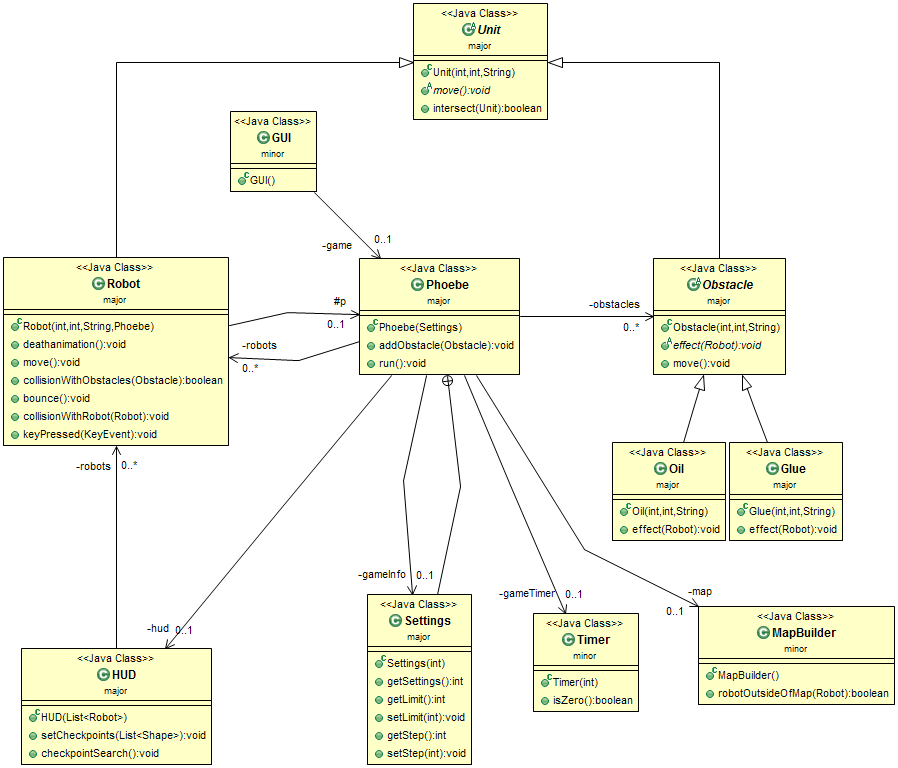
\includegraphics[width=17cm]{images/struktdiagram.PNG}
\caption{Statikus struktúra diagram}
\label{fig:example3}
\end{center}
\end{figure}
\pagebreak


\section{Osztályok leírása}

\subsection{Cleaner}
\begin{itemize}
\item Felelősség\\

\item Ősosztályok\\
Unit$\rightarrow$Robot
\item Attribútumok
    \begin{itemize}
        \item List obstacles:  
    \end{itemize}
\item Metódusok
	\begin{itemize}
	    \item \textbf{Cleaner}(int x, int y, Phoebe p):
		\item void \textbf{setObstacles}(List obsts): 
		\item boolean \textbf{collisionWithRobot}():
		\item void \textbf{collisionWithCleaner}():
		\item void \textbf{move}():
	\end{itemize}
\end{itemize}



\subsection{GUI}
\begin{itemize}
\item Felelősség\\
A grafikus felületért felelős osztály, amely a menüt és a játékot jeleníti meg.
\item Attribútumok
	\begin{itemize}
		\item \textbf{Phoebe} game: referencia a játékra
	\end{itemize}
\item Metódusok
	\begin{itemize}
		\item\textbf{GUI}(): Konstruktor. Beállítja az ablak nevét, létrehozza az ablak elemeit, elrendezi őket és beállítja a figyelőket(ActionListener).
	\end{itemize}
\end{itemize}

\subsection{HUD}
\begin{itemize}
\item Felelősség\\
A robotok megtett köreit és checkpontjait tartja számon. Megvalósítja a checkpoint ellenőrzést.
\item Attribútumok
	\begin{itemize}
		\item \textbf{int[]} checkpointReached: Minden robothoz külön tárolja a legutoljára érintett checkpoint sorszámát.
		\item \textbf{int[]} lap: Minden robothoz tárolja a megtett körök számát. 
		\item \textbf{List} checkpoints: Tárolja a checkpointokat reprezentáló objektumokat List adatszerkezetben. A checkpointSearch függvény kérdezi le ebből a következő checkpoint helyzetét. 
		\item \textbf{List<Robot>} robots: A robotokat tároló List adatszerkezet. A checkpointSearch függvény kérdezi le ebből a robotokat, majd azok helyzetét.
	\end{itemize}
\item Metódusok
	\begin{itemize}
		\item \textbf{HUD}(List<Robot> robs): Robot objektumokat tároló ArrayList. Célja, hogy a checkpointsearch() függvényben minden robotra elvégezzük a keresést.
		\item void \textbf{checkpointSearch}(): Minden híváskor ellenőrzi, hogy a robot és a checkpoint metszete üres-e. 
		\item int \textbf{endOfTheGame}(): A játék végén eldönti, hogy melyik játékos nyert. Visszatér egy számmal, amiből egyértelműen eldönthető, hogy ki nyert. Ha negatív akkor az 1-es számú játékos nyert, ha nulla akkor döntetlen, ha pozitív akkor a 2-es számú játékos nyert.
		\item void \textbf{setCheckpointReached}(Robot r): Ha a paraméterként átadott robot következő checkpointja a célvonal (utolsó checkpoint) akkor lenullázza a checkpointReached-et és növeli a megtett körök számát, illetve ha nem akkor növeli az érintett checkpointok számát.
		\item void \textbf{setCheckpoints}(List checkObj): Checkpointokat reprezentáló adatszerkezet betöltése.CheckpointReached inicializálása a checkpointok számától függően.
	\end{itemize}
\end{itemize}

\subsection{IVisible}
\begin{itemize}
\item Felelősség\\
A grafikus motorhoz szükséges interfész. Olyan osztályok, melyek kirajzolható elemeket tartalmaznak megvalósítják ezt az interfészt.
\item Metódusok
	\begin{itemize}
		\item void \textbf{paint}(Graphics2D g): Rajzolást elvégző metódus.
	\end{itemize}
\end{itemize}

\subsection{List}
\begin{itemize}
    \item Felelősség
        \begin{itemize}
        \item Objektumok tárolása, ezt az interfészt megvalósító osztályban.
        \item \url{https://docs.oracle.com/javase/6/docs/api/java/util/List.html}
        \end{itemize}
\end{itemize}

\subsection{MapBuilder}
\begin{itemize}
\item Felelősség\\
A pálya felépítéséért, a checkpointok tárolásáért és a robot pályán tartózkodásának vizsgálatáért felelős osztály.
\item Attribútumok
	\begin{itemize}
		\item \textbf{List} checkpoints: Tárolja a checkpointokat reprezentáló objektumokat List adatszerkezetben.
		\item \textbf{Object} map: A pályát reprezentáló objektum.
		\item \textbf{int[]} startPosPlayerOne: Meghatároz egy (x,y) koordinátát, ahol az első játékos kezd.
		\item \textbf{int[]} startPosPlayerTwo: Meghatároz egy (x,y) koordinátát, ahol az második játékos kezd.
	\end{itemize}
\item Metódusok
	\begin{itemize}
		\item \textbf{MapBuilder}(): Konstruktor, a pálya beolvasása fájlból, majd létrehozása.
		\item int[] \textbf{getStartPosPlayer}(int id): Paraméterül kap egy Robot id-t, majd visszatér egy int tömbbel, melyben található a robot kezdőpozíciója a pályán.
		 \item boolean \textbf{obstacleOutsideOfMap}(Obstacle obs): Egy akadályt vizsgál, hogy a pályán van-e.
		\item boolean \textbf{robotOutsideOfMap}(Robot r): Igaz értéket ad vissza, ha a robot leesett a pályáról, hamisat ha még rajta van.
	\end{itemize}
\end{itemize}

\subsection{MyListener}
\begin{itemize}
\item Felelősség\\
A külön szálon futó KeyListener-t megvalósító osztály.
\item Interface-ek:
    \begin{itemize}
    \item KeyListener
    \item Runnable
    \end{itemize}
\item Attribútumok
	\begin{itemize}
		\item -\textbf{boolean} isUp: Azt tárolja, hogy le van-e nyomva a felfele nyil.
    	\item -\textbf{boolean} isDown: Azt tárolja, hogy le van-e nyomva a lefele nyil.
    	\item -\textbf{boolean} isRight:Azt tárolja, hogy le van-e nyomva a jobbra nyil.
    	\item -\textbf{boolean} isLeft:Azt tárolja, hogy le van-e nyomva a balra nyil.
    	\item -\textbf{boolean} isW:Azt tárolja, hogy le van-e nyomva a W a billentyűzeten.
    	\item -\textbf{boolean} isD:Azt tárolja, hogy le van-e nyomva a D a billentyűzeten.
    	\item -\textbf{boolean} isS:Azt tárolja, hogy le van-e nyomva az S a billentyűzeten.
    	\item -\textbf{boolean} isA:Azt tárolja, hogy le van-e nyomva az A a billentyűzeten.
   	\item -\textbf{List<Robot>} robots: Azon robotok listája akiknek a keyPressed függvényét kell hívnia.
	
	
	\end{itemize}
\item Metódusok
	\begin{itemize}
		\item+ \textbf{MyListener}(List<Robot> r): beállítja a lenyomott gombokat figyelő változókat false-ra , továbbá beállítja a robots változó referenciáját a paraméterként kapotra.
			\item+ void\textbf{keyPressed}(KeyEvent e): Beállítja a lenyomot gombokat figyelő változók küzül a Keyeventnek megfelelőt  true-ra , ha meg nyomták valamelyiket  a figyelt gombok közül.
			\item+ void\textbf{keyReleased}(KeyEvent e): Beállítja a lenyomot gombokat figyelő változók küzül a Keyeventnek megfelelőt false-ra , ha fel engedték valamelyiket a figyelt, lenyomott gombok közül.
				\item+ void\textbf{run}(): Végtelen ciklust futtat. Megvizsgálja hogy melyik gombok vannak lenyomva, majd a nekik megfelelő KeyEvent-tel paraméterezve meghívja a hozzátartozó robotoknak a Keypressed függvényét. Majd alszik a szál 30 mili secundomig.
	\end{itemize}
\end{itemize}

\subsection{MyTimer}
\begin{itemize}
\item Felelősség\\
A játék elején a kezdésig visszaszámol három másodpercet, utána indulhat a játék. Játéktípustól függően felfelé(kör játékmód) vagy visszafelé(idő játékmód) számol. Ez az osztály felelős, azért ha lejár az idő vége legyen a játéknak,
\item Attribútumok
    \begin{itemize}
        \item - enum DIR: Az óra számolási irányának enumerizácciója.
        \item - long T\_start: Az óra indításának időpontja millisec pontosággal.
	    \item - int duration: Ha az óra visszafelé számol, akkor tárolja, hogy mennyi volt a kezdő érték, ha felfelé számol, akkor értéke 0. Mértékegysége millisekundum.
	    \item - DIR direction: Az óra számolási irányának eltárolásáért felelős enum.
    \end{itemize}
\item Metódusok
	\begin{itemize}
		\item + \textbf{MyTimer}(int i): Konstruktor. Ha 0-val vagy negatívval inicializálják felfele számol, ha pozitív számmal inicializálják akkor lefelé számol.
		\item + boolean \textbf{isZero}(): Az idő lejárását ellenörző függvény, megadja, hogy az indítás plusz a megadott időtartam kisebb-e a pillanatnyi időnél.
		\item + int \textbf{getTime}():  Ha pozitív száámal inicializálódott az objektum, akkor megadja mennyi idő van még hátra a visszaszámlálásból vagy, ha nullával, akkor a start() hívás óta eltelt idővel tér vissza.
		\item + void \textbf{start}(): Az óra indításakor vagy újraindításakor meghívott függvény. Csak akkor indul újra (visszaszámláló üzemmódban), ha elérte a 0-t. A Phoebe run() metódusa hívja meg, mikor vissza kell számolni a játék kezdete előtt három másodpercet. Illetve, a játék kezdetekor.
	\end{itemize}
\end{itemize}

\subsection{Obstacle}
\begin{itemize}
\item Felelősség\\
A pályán/játékosoknál lévő különböző akadályokat (ragacs,olaj) összefogó ősosztály.
\item Ősosztályok\\
Unit
\item Attribútumok
	\begin{itemize}
		\item \# \textbf{int} WIDTH: Az akadályokat jellemző szélesség. Szükség van rá, hogy létrehozzuk a leszármazottak hitbox-át(sokszög pályaelem).
		\item \# \textbf{int} HEIGHT: Az akadályokat jellemző hosszúság. Szükség van rá, hogy létrehozzuk a leszármazottak hitbox-át(sokszög pályaelem).
			\item \# \textbf{int} lifetime: Generikussan az akadályok életben maradásának ellenörzésére szolgál. Olaj esetében megadja, hogy hány kör telt el az akadály lerakása óta. Ragacs esetében pedig, hogy hányan léptek rá mióta lekerült. 
	\end{itemize}
\item Metódusok
	\begin{itemize}
		\item +\textbf{Obstacle}(int x, int y): meghívja a Unit konstruktorát a megadott adatokkal és létrehoz egy négyzet elemet ami reprezentálja a pályán majd.
		\item + void \textbf{effect}(Robot r): Meghatározza, milyen hatással van a robotra, ha érintkezik egy Obstacle-lel. Absztrakt.
		\item +boolean \textbf{checkAlive}():Az akadályok vizsgálata amit a játékmotor minden körben meghív minden akadályra. Absztrakt.
	\end{itemize}
\end{itemize}

\subsection{Glue}
\begin{itemize}
\item Felelősség\\
A játékban szereplő Ragacs foltok viselkedését leíró osztály
\item Ősosztályok\\
Unit$\rightarrow$Obstacle
\item Attribútumok
	\begin{itemize}
		\item -\textbf{BufferedImage} img: Ez a  statikus atribútum a ragacs képét tárolja,  a megjelenítésben van szerepe.
	\end{itemize}
\item Metódusok
	\begin{itemize}
		\item  \textbf{Glue}(int x,int y):A ragacs konstruktora, meghívja az őse (obstacles)                           konstruktorát x,y paraméterrel, továbbá beállítja a lifetime-ot 4-re.
		
		\item+ void \textbf{effect}(Robot r): Ütközéskor hívja meg az ütközést vizsgáló függvénye     a Robot osztálynak. Módosítja a robot slowed értékét a 50\%-ra a robot slowed attribútum         setterének meghívásával. Továbbá csökkenti a ragacs élettartalmát egyel.
	
		\item+ boolean \textbf{checkAlive}():A játékmotor hívja meg minden kör végén, ha a lifetime értéke>0 true-val tér vissza, különben false-al.
			\item+ void \textbf{paint}(Graphics2D g):Kirajzolja a ragacs képét az x,y koordinátákon.
				\item+ void \textbf{setUnitImage}():Beállítja a ragacs osztályhoz tartozó képet a user directoryban található glue.jpg-re
			\item+ String \textbf{toString}()Vissza ad egy stringet a  ragacs legfontosabb értékeivel.(x, y, WIDTH, HEIGHT, lifetime)
		
	\end{itemize}
\end{itemize}

\subsection{Oil}
\begin{itemize}
\item Felelősség\\
A pályára lerakható olaj megvalósítása. Ha belelép egy játékos egy ilyen olajfoltba az effect függvény letiltja a mozgatást az adott roboton a következő ugrásig.
\item Ősosztályok\\
Unit $\rightarrow$ Obstacle 
\item Attribútumok
	\begin{itemize}
		\item- \textbf{BufferedImage} img: Ez a  statikus atribútum az olaj képét tárolja,  a megjelenítésben van szerepe.
	\end{itemize}
\item Metódusok
	\begin{itemize}
		\item + \textbf{Oil}(int x, int y): Egy Oil elem létrehozásáért felelős. Meghívja az ős konstruktorát x,y-paraméterrel, továbbá beállítja a lifetime-ot default értékre.
		\item + void \textbf{effect}(Robot r): Meghatározza, milyen hatással van a robotra, ha beleugrik egy olajfoltba. Ebben az esetben letiltja a játékost, hogy irányt váltson.
			\item + void \textbf{setUnitImage}():Beállítja az olaj osztályhoz tartozó képet a user directoryban található oil.jpg-re
				\item + boolean \textbf{checkAlive}():A játékmotor hívja meg minden kör végén, lifetime értékét csökkenti 1 el, ha a lifetime értéke>0 (csökkentés után)true-val tér vissza, különben false-al.
		\item + String \textbf{toString}()Vissza ad egy stringet az olaj legfontosabb értékeivel.(x, y, WIDTH, HEIGHT, lifetime)
	\end{itemize}
\end{itemize}

\subsection{Phoebe}
\begin{itemize}
\item Felelősség\\
A játék motorját megvalósító objektum. Listában tárolja a pályán tartózkodó robotokat,kisrobotokat, akadályokat és 
 figyeli, hogy mikor ér véget a játék. A „Phoebe” objektum rajzolja ki az objektumokat a pályán és 
 szálként indítható osztályt, melyben maga a játék fut. Játékindításkor berakja a pályára a robotokat és 
 az akadályokat a kezdő pozíciókba. Ebben az objektumban történnek az ellenőrzések (akadályba vagy 
  robotba ütközések, pályáról leesés)
  \item Interface:
  \begin{itemize}
  \item Runnable
  \end{itemize}
\item Attribútumok
	\begin{itemize}
		\item- \textbf{boolean} ended: Állapot változó, ha vége a játéknak, akkor true. Ha beteljesül egy játék végét jelentő esemény, akkor ezen a változón keresztül leáll a játék és megállapítódik a nyertes.
		\item+ \textbf{BufferedImage} background: A játék hátterét adó kép.
		\item- \textbf{List<Robot>} robots: A játékban szereplő robotok listája.
		\item- \textbf{List<Obstacle>} obstacles: A játékban szereplő akadályok listája.
		\item- \textbf{HUD} hud: A játékosok előrehaladását, ragacs és olajkészleteit tartja számon
		\item- \textbf{MapBuilder} map: TODO
		\item- \textbf{Settings} gameInfo:A játék beállításait tartalmazza         \item- \textbf{List<Cleaner>} cleaners: A játékban lévő aktív kis tisztogató robotokat tartja számon.
        \item- \textbf{MyTimer} gameTimer: A játékban futó óra, ami visszaszámlálásoknál és a játék végének meghatározásánál játszik szerepet.

		
			
	\end{itemize}
\item Metódusok
	\begin{itemize}
		\item+ \textbf{Phoebe}(Setting set): A játék felépítése, a robotok,a tisztogató kisrobotok és  az akadályok listáinak létrehozása.Az ended inicializálása ,az init függvény meghívása és a grafikus felület felépítése történik itt.
		\item+ void \textbf{run}(): Ez a metódus futtatja a főciklust, amelyben maga a játék működik.
	\item+ void \textbf{Paint}(Graphics2D g2d): Kirajzolja a játék aktuális állását. 
	\item+ void \textbf{addObstacle}(Obstacle item): Hozzá ad egy Obstacle-t a játékban lévők listájához.
	
	\item- void \textbf{init}(): Inicializálja a játékot a kezdeti beállításokra. Létrehozza az időzítőt, a mapot, a robotokat a kezdőpozíciók szerint,a hudot és beállítja a különböző osztályokhoz tartozó statikus képeket, továbbá a pálya alap ragacsait és olajait is szétszórja.
	\end{itemize}
\end{itemize}

\subsection{Robot}
\begin{itemize}
\item Felelősség\\
A játékban résztvevő ugráló robotok viselkedését és kezelését leíró osztály, tárolja és kezeli a felhasználható akadályok számát.
  Olyan objektum, mely a pályán található robotokat valósítja meg. Leírja a viselkedésüket és a kezelésüket. 
  A „Robot” osztály a Unit-ból származik le, ezáltal van pozíciója és az ütközés is le van kezelve. 
  Felelős a mozgásért, megállapítja egy adott akadállyal vagy robottal ütközött-e és kezeli a felhasználó által leütött gombokat.
  \item Ősosztályok\\
Unit

\item Attribútumok
	\begin{itemize}
		\item\# \textbf{int} staticID: Az osztályhoz tartozó statikus azonosító, a példány                azonosítójának(id) meghatározásához szükséges.
			\item- \textbf{static final int} r: Az ugrás számításához tartozó sugár. 
				\item- \textbf{static final int} ANIMATIONSPEED: Az ugrás animálásának részletessége(hányszor hívja meg a paintet). 
		\item\# \textbf{static int} HEIGHT: A robot képének magassága, collision                      detektálásnál, továbbá az irányítást segítő nyíl kezdő koordinátájának                  meghatározásánál szükséges.
		\item\# \textbf{static int} WIDTH:A robot képének szélessége, funkcionalitásban hasonló a WIDTH-hez.
		\item- \textbf{int} ID: A robot példányának egyedi azonosítója, a keyconfig sorának                     indexelésére és a collison detektálásnál az önmagával való ütközés                      kivédésére szükséges.
		\item- \textbf{int} numGlue:A robotnál lévő ragacskészletet tárolja.
		\item- \textbf{int} numOil:A robotnál lévő olajkészletet tárolja.
		\item- \textbf{boolean} leftobstacle:Megmondja hogy raktunk-e már le ebben a körbe olajat vagy ragacsot kezdő érték false, minden lépés után vissza áll false ra és minden obstacle lerakásnál true ra .
	\item\# \textbf{BufferedImage}img[]:A robotok képeit tartalmazza,az animáció miatt többet.
	
		\item- \textbf{double} slowed: A sebesség modosításáért felel, default értéje 1.0, amennyiben ragacsba lép a robot ez 0.5-re módosul és minden ugrás végén visszaáll az eredeti értékére, ugrásnál ezzel szorozzuk be a végkordinátát kiszámító sugár hosszát.
		\item- \textbf{boolean} oiled: Azt jelzi, hogy olajba lépett-e, ennek hatására a mozgás iránya módosíthatatlanná válik egy kis időre. 
		\item\# \textbf{int} arrowendx: A robot irányítását segítő nyilnak az x koordinátája, a nyíl kirajzolásánál van szerepe.
		\item\# \textbf{int} arrowendy: A robot irányítását segítő nyilnak az y koordinátája, a nyíl kirajzolásánál van szerepe.
		\item- \textbf{double} alpha: A robot irányítását segítő nyíl vízszintessel bezárt szöge. A nyil kirajzolásánál, az ugrás végpontjának meghatározánál van szerepe.
		\item\# \textbf{boolean} moved: Azt jelöli, hogy lépett-e már a robot az aktuális körben. A megjelenítésnél(nyilat ugrás közben nem jelenítjük meg),illetve az irányítás letiltásánál van szerepe(olajba lépés esetén).
	
\end{itemize}
\item Metódusok\\
	\begin{itemize}
		\item+ \textbf{Robot}(int x,int y,Phoebe p): Létrehoz egy robotot a megadott x,y kordinátákon, inicializálja a tagváltozóit és eltárolja a játékmotor referenciáját.
		\item+ void\textbf{deathanimation}():A Robot halálának gafikus megjelenítéséért felelős függvény.
		\item+ void\textbf{setOiled}():Az oiled értékét true-ra állítja. 
		\item+ void\textbf{setGlued}():A slowed értékét 0.5-re állítja. 
		\item+ int\textbf{getId}():A Robot id-ét adja vissza.
		\item+ int\textbf{getNumGlue}():Visszatér a felhasználható ragcsok számával.
		\item+ int\textbf{getNumOil}():Visszatér a felhasználható olajok számával.
		\item+ void\textbf{incNumOil}():Növeli a robotnál tárolt olajok számát, ha az nem haladja meg a 3 at.
		\item+ void\textbf{incNumGlue}():Növeli a robotnál tárolt ragacsok számát, ha az nem haladja meg a 3 at.
	\item+ void\textbf{paint}(Graphics2D g):kirajzolja a robotot a saját koordinátáin, ha nem lép éppen akkor az irányítást segítő nyilat is.
	\item+ void\textbf{setUnitImage}():beállítja a robot osztályhoz tartozó képeket.
\item+ void\textbf{bounce}():A robotok ütközésekor a lepattanás céjának  koordinátáinak számolása történik itt.

		\item+ void\textbf{move}():A robot mozgatásáért és annak leanimálásáért felelős függvény.Kiszámolja az új koordinátát és oda ugrasztja a robotot, majd frissíti a hitboxot.
		\item+ boolean \textbf{collisionWithObstacle}(Obstacle o): Ellenőrzi hogy a robot ütközött-e az akadállyal, igazzal tér vissza ha igen, hamissal ha nem.
		\item+ boolean \textbf{collisionWithRobot}(Robot r): Ellenőrzi hogy a robot ütközött-e másik robottal ,  referencia alapján kiszüri ha önmagára hívják meg.Ha volt ütközés meghívja a bounce függvényt önmagára.Igazzal tér vissza ha volt ütközés és hamissal ha nem.
		\item+ void \textbf{keyPressed}(int e):A robot irányítását megvalósító függvény, a játékmotor keylistener-e által hívódik meg, a lenyomott billentyű azonosítójával. A következő ugrás beállítása, a ragacs/olaj lerakása történhet itt. A Settings.keyconfig változó felhasználásával.
				\item+ String \textbf{toString}()Vissza ad egy stringet a robot legfontosabb értékeivel.(id, slowed, oiled, x, y, nextx, nexty, alpha, WIDTH, HEIGHT, numGlue, numOil)
	\end{itemize}
\end{itemize}

\subsection{Unit}
\begin{itemize}
\item Felelősség\\
A pályán található objektumokért felel és azok viszonyáról (például ütközésükről).
\item Attribútumok
	\begin{itemize}
		\item \# \textbf{Object} hitbox: Az egységet a pályán reprezentáló sokszög.
		\item \# \textbf{int} x: Az egység x koordinátája
		\item \# \textbf{int} y: Az egység y koordinátája
	\end{itemize}
\item Metódusok
	\begin{itemize}
	    \item + \textbf{Unit}(): A Unit osztály konstruktora. Feladata, hogy eltárolja az x,y koordinátát.
		\item + boolean \textbf{intersect}(Unit u): Két egység ütközését meghatározó függvény.
		\item + void \textbf{move}() : Absztrakt függvény, mely a leszármazottakban fog megvalósulni. Az egységek mozgásáért felelős.
	\end{itemize}
\end{itemize}

\section{A tesztek részletes tervei, leírásuk a teszt nyelvén}
[A tesztek részletes tervei alatt meg kell adni azokat a bemeneti adatsorozatokat, amelyekkel a program működése ellenőrizhető. Minden bemenő adatsorozathoz definiálni kell, hogy az adatsorozat végrehajtásától a program mely részeinek, funkcióinak ellenőrzését várjuk és konkrétan milyen eredményekre számítunk, ezek az eredmények hogyan vethetők össze a bemenetekkel.]

\subsection{Teszteset1}
\begin{itemize}
\item Leírás\newline
\comment{szöveges leírás, kb. 1-5 mondat.}
\item Ellenőrzött funkcionalitás, várható hibahelyek
\item Bemenet\newline
\comment{a proto bemeneti nyelvén megadva (lásd előző anyag)}
\item Elvárt kimenet\newline
\comment{a proto kimeneti nyelvén megadva (lásd előző anyag)}
\end{itemize}

\subsection{CollisionWithRobot\_VOLTÜTKÖZÉS\_TESZT}
\begin{itemize}
	\item Leírás: Ez a teszt a collisionWithRobot(Robot r) függvény teszteléséért felelős.
			Létrehoz 2 robotot majd beállítja az őket, úgy hogy egymásra ugorjanak .
			Kiirja az adataikat  és meghivja a move függvényt ezt követően pedig az egyik collisionWithRobot függvényét a másikra	és újból ki listáza őket.	\newline
	\item Ellenőrzött funkcionalitás, várható hibahelyek: Azt ellenörizzük hogy sikeressen össze tudta-e vetni a hitboxokat a függvény az ugrás végeztével .
	Várható hiba ha hamissal tér vissza a függvény, amiből látjuk, hogy rossz a hitbox létrehozása az új helyen az ugrást követően.
	\item Bemeneti nyelv :
		\begin{itemize}
		\item Robot(500,500)
		\item Robot(600,400)
		\item Keypressed(Keyevent.VK\_A,90)
		\item listRobots
		\item move
		\item listRobots
		\end{itemize}

	\item Elvárt kimenet: \\
		"Robot [id=0,  slowed=1,oiled=false, x=500,y=500, 
		\\numGlue=3,numOil=3,nextx=500,
		\\nexty=400,alpha=1.57,width=40,height=40]"\newline
		"Robot [id=1,  slowed=1,oiled=false, x=600,y=400, 
		\\numGlue=3,numOil=3,nextx=600,
		\\nexty=300,alpha=1.57,width=40,height=40]"
		
		"nextx ,nexty modified to:500,400"
	
		"Robot [id=0,  slowed=1,oiled=false, x=500,y=500, 
		\\numGlue=3,numOil=3,nextx=500,
		\\nexty=400,alpha=1.57,width=40,height=40]"\newline
		"Robot [id=1,  slowed=1,oiled=false, x=600,y=400, 
		\\numGlue=3,numOil=3,nextx=500,
		\\nexty=400,alpha=1.57,width=40,height=40]"

		 "there was a collision between this: "Robot [id=0,  slowed=1,oiled=false, x=500,y=400, 
		\\numGlue=3,numOil=3,nextx=500,
		\\nexty=400,alpha=1.57,width=40,height=40]"\newline
		and this:
		"Robot [id=1,  slowed=1,oiled=false, x=500,y=400, 
		\\numGlue=3,numOil=3,nextx=500,
		\\nexty=150,alpha=3.04,width=40,height=40]"\newline
		
	    "Robot [id=0,  slowed=1,oiled=false, x=500,y=400, 
		\\numGlue=3,numOil=3,nextx=500,
		\\nexty=400,alpha=1.57,width=40,height=40]"\newline
		
		"Robot [id=1,  slowed=1,oiled=false, x=500,y=400, 
		\\numGlue=3,numOil=3,nextx=500,
		\\nexty=150,alpha=3.04,width=40,height=40]"\newline

\end{itemize}
\subsection{CollisionWithRobot\_NEMVOLTÜTKÖZÉS\_TESZT}
\begin{itemize}
	\item Leírás: Ez a teszt a collisionWithRobot(Robot r) függvény teszteléséért felelős.
			Létrehoz 2 robotot  .
			Kiirja az adataikat  és meghivja a move függvényt ezt követően pedig az egyik collisionWithRobot függvényét a másikra 
			és újból ki listáza őket.			\newline
	\item Ellenőrzött funkcionalitás, várható hibahelyek: Azt ellenörizzük hogy sikeressen össze tudta-e vetni a hitboxokat a függvény az ugrás végeztével .
	Várható hiba ha loggol collisiont a függvény, amiből látjuk, hogy rossz a hitboxok össze vetése , hisz nem lehet ütközés. 
	\comment{\\Ctrl-C, Ctrl-V hiba, most akkor mivel kell visszatérnie. \\ \\Kellene logolni a collisionWithRobot() kimenetelét, a függvényen belül? by Don.\\
	most úgy van a függvény hogy van visszatérési értéke ... így könnyebb lesz majd égetve logolni a teszten belül , de akár a belselyébe is be lehet rakni a kiirást( de multkor azt beszéltük hogy ha nincs log az is log (a collision kiirásának elmulasztása felér azzal hogy nem volt collision))}
	
	\comment{Hát nem tudom mi lenne jobb. Ennél a két tesztesetnél jó lenne látni, hogy megtörtént a vizsgálat és az eredményét.}
	
	\item Bemeneti nyelv :
		\begin{itemize}
		\item Robot(500,500)
		\item Robot(600,400)
		\item listRobots
		\item move
		\item listRobots
		\end{itemize}
	

	\item Elvárt kimenet: \\
		"Robot [id=0,  slowed=1,oiled=false, x=500,y=500, 
		\\numGlue=3,numOil=3,nextx=500,
		\\nexty=400,alpha=1.57,width=40,height=40]"\newline
		"Robot [id=1,  slowed=1,oiled=false, x=600,y=400, 
		\\numGlue=3,numOil=3,nextx=600,
		\\nexty=300,alpha=1.57,width=40,height=40]"
		
		
		\comment{most akkor merre ugrik? \\0.állapot Robot0(500,500)->(500,400),Robot1(600,400)->(600,300) \\1. állapot Robot0(500,400)->(400,400),Robot1(600,400)->(600,400)\\Figyelj arra is, hogy a nextx, nexty megfelelően értékbe álljanak, ne váltson irányt a Robot0. by Don}
		\comment {ehez volna jó ha működne a grafikus felület mert eléggé bele tudok zavarodni a monitor képpont indexelésébe}
		
		
		 "Robot [id=0,  slowed=1,oiled=false, x=500,y=400, 
		\\numGlue=3,numOil=3,nextx=500,
		\\nexty=400,alpha=1.57,width=40,height=40]"\newline
		"Robot [id=1,  slowed=1,oiled=false, x=600,y=300, 
		\\numGlue=3,numOil=3,nextx=600,
		\\nexty=300,alpha=1.57,width=40,height=40]"\newline
		
\end{itemize}

\subsection{CollisionWithRobot\_IRÁNYVÁLTOZTATÁS\_TESZT}
\begin{itemize}
	\item Leírás: Ez a teszt a KeyPressed(int e) függvény teszteléséért felelős.
			Létrehoz 2 robotot.
			Kiirja az adataikat  és meghivja a KeyPressed(int e)  függvényt VK\_D és VK\_LEFT paraméterekkel majd meghívjuk a move-ot és újból ki listáza őket. A várt eredmény, hogy 180 fokban elfordultak és úgy léptek.			\newline
	\item Ellenőrzött funkcionalitás, várható hibahelyek: Azt ellenörizzük hogy sikeressen ki tudta e számolni a függvény az új koordinátákat.
		Várható hiba hogy rosszul modosítja a cél koordinátákat vagy az alpha szöget. 
		Ezt onnan látjuk, hogy nem a várt koordinátákat látjuk a nextx, nexty, alpha tagváltozókban miután másodjára is kilistáztuk őket vagy mikor a keypressed kiirja.
	\item Bemeneti nyelv :
		\begin{itemize}
		\item Robot(500,500)
		\item Robot(600,400)
		\item listRobots
		\item Keypressed(Keyevent.VK\_A,180)
		\item Keypressed(Keyevent.VK\_LEFT,180)
		\item move
		\item listRobots
		\end{itemize}
	
	\item Elvárt kimenet: \\
		"Robot [id=0,  slowed=1,oiled=false, x=500,y=500, 
		\\numGlue=3,numOil=3,nextx=500,
		\\nexty=600,alpha=1.57,width=40,height=40]"\newline
		"Robot [id=1,  slowed=1,oiled=false, x=600,y=400, 
		\\numGlue=3,numOil=3,nextx=600,
		\\nexty=500,alpha=1.57,width=40,height=40]"\newline
		
		"nextx ,nexty modified to:500,400"\\
		"nextx ,nexty modified to:600,300"\\
	\comment{Ne felejtsd, hogy a keypressed állítja az alpha-t is! Illetve a Robotok magukba fognak ??miért???? ugrani(500,400)->(500,400), (600,300)->(600,300). by Don}\\
		"Robot [id=0,  slowed=1,oiled=false, x=500,y=400, 
		\\numGlue=3,numOil=3,nextx=500,
		\\nexty=400,alpha=4.71238898,width=40,height=40]"\newline
		"Robot [id=1,  slowed=1,oiled=false, x=600,y=300, 
		\\numGlue=3,numOil=3,nextx=600,
		\\nexty=300,alpha=4.71238898,width=40,height=40]"\newline
\end{itemize}

\subsection{robotOutsideOfMap\_A.PÁLYÁRÓL.LEESETT\_TESZT}
\begin{itemize}
	\item Leírás: Ez a teszt a robotOutsideOfMap(Robot r) függvény teszteléséért felelős.
			Létrehoz 1 robotot majd beállítja, úgy hogy kiugorjon a pályáról .
			Kiirja az adatait  és meghivja a move függvényt ezt követően pedig a robotOutsideOfMap függvényt és leellenőrizzük hogy a listában maradt-e a robot.	\newline
	\item Ellenőrzött funkcionalitás, várható hibahelyek: Azt ellenörizzük hogy sikeressen össze tudta-e vetni a hitboxokat a függvény az ugrás végeztével .
	Várható hiba ha hamissal tér vissza a függvény, amiből látjuk, hogy rossz a hitbox létrehozása  az ugrást követően.
	\item Bemeneti nyelv :
		\begin{itemize}
\item MapBuilder map
		\item Robot(400,500)
		\item listRobots
		\item Keypressed(Keyevent.VK\_A,90)
		\item move
		\item listRobots
		\end{itemize}

	\item Elvárt kimenet: \\
		"Robot [id=0,  slowed=1,oiled=false, x=400,y=500, 
		\\numGlue=3,numOil=3,nextx=400,
		\\nexty=400,alpha=1.57,width=40,height=40]"\newline
		
		"nextx ,nexty modified to:400,400"\newline
	
		"Robot [id=0,  slowed=1,oiled=false, x=400,y=500, 
		\\numGlue=3,numOil=3,nextx=400,
		\\nexty=400,alpha=1.57,width=40,height=40]"\newline
		 
		 "there was a collision between this: "Robot [id=0,  slowed=1,oiled=false, x=500,y=400, 
		\\numGlue=3,numOil=3,nextx=500,
		\\nexty=400,alpha=1.57,width=40,height=40]"\newline
		and this:
		"Map"\newline
		
	    "-"\comment{Nincs a robot a listában.}\newline 
\end{itemize}

\subsection{robotOutsideOfMap\_NEM.ESETT.LE.PÁLYÁRÓL\_TESZT}
\begin{itemize}
	\item Leírás: Ez a teszt a robotOutsideOfMap(Robot r) függvény teszteléséért felelős.
			Létrehoz 1 robotot majd beállítja, úgy hogy ne ugorjon ki a pályáról .
			Kiirja az adatait  és meghivja a move függvényt ezt követően pedig a robotOutsideOfMap függvényt és leellenőrizzük hogy a listában maradt-e             a robot.\newline
	\item Ellenőrzött funkcionalitás, várható hibahelyek: Azt ellenörizzük hogy sikeressen össze tudta-e vetni a hitboxokat a függvény az ugrás                     végeztével .
	        Várható hiba ha igazzal tér vissza a függvény, amiből látjuk, hogy rossz a hitbox létrehozása  az ugrást követően.
	\item Bemeneti nyelv :
		\begin{itemize}
\item MapBuilder map
		\item Robot(400,500)
		\item listRobots
		\item Keypressed(Keyevent.VK\_D,90)
		\item move
		\item listRobots
		\end{itemize}

	\item Elvárt kimenet: \\
		"Robot [id=0,  slowed=1,oiled=false, x=400,y=500, 
		\\numGlue=3,numOil=3,nextx=400,
		\\nexty=600,alpha=1.57,width=40,height=40]"\newline
		
		"nextx ,nexty modified to:400,600"\newline
		
		"-"\comment{Nem történt ütközés a robot és a pálya között}\newline
	
		 "Robot [id=0,  slowed=1,oiled=false, x=400,y=500, 
		\\numGlue=3,numOil=3,nextx=400,
		\\nexty=600,alpha=1.57,width=40,height=40]"\newline
	
\end{itemize}


\subsection{checkpointSearch\_CHEICKPOINTONBA.UGRÁS\_TESZT}
\begin{itemize}
	\item Leírás: Ez a teszt a checkpointSearch() függvény teszteléséért felelős.
			Létrehoz 1 robotot majd beállítja, úgy hogy ugorjon bele a checkpointba.
			Kiirja az adatait  és meghivja a move függvényt ezt követően pedig a checkpointSearch függvényt és leellenőrizzük hogy van-e a két hitboxnak metszette.\newline
	\item Ellenőrzött funkcionalitás, várható hibahelyek: Azt ellenörizzük hogy sikeressen össze tudta-e vetni a hitboxokat a függvény az ugrás                     végeztével .
	        Várható hiba ha hamissal tér vissza a függvény, amiből látjuk, hogy rossz a hitbox létrehozása  az ugrást követően.
	\item Bemeneti nyelv :
		\begin{itemize}
\item MapBuilder map
        \item MapBuilder Map
        \item setCheckpoints 100,180
		\item Robot(100,100)
		\item listCheckpoints
		\item listRobots
		\item Keypressed(Keyevent.VK\_D,90)
		\item move
		\item listRobots
		\end{itemize}

	\item Elvárt kimenet: \\
	    "Checkpoint: 100,180"\newline
	    
		"Robot [id=0,  slowed=1,oiled=false, x=100,y=100, 
		\\numGlue=3,numOil=3,nextx=100,
		\\nexty=200,alpha=1.57,width=40,height=40]"\newline
		
		"nextx ,nexty modified to:100,200"\newline
		
		 "there was a collision between this: Robot [id=0,  slowed=1,oiled=false, x=100,y=200, 
		\\numGlue=3,numOil=3,nextx=100,
		\\nexty=200,alpha=1.57,width=40,height=40]
		\\and this: 
		  Checkpoint: 100,180"\newline
	
		 "Robot [id=0,  slowed=1,oiled=false, x=100,y=200, 
		\\numGlue=3,numOil=3,nextx=100,
		\\nexty=200,alpha=1.57,width=40,height=40]"\newline
	
\end{itemize}

\subsection{checkpointSearch\_CHEICKPOINTONBA.NEM.UGRÁS\_TESZT}
\begin{itemize}
	\item Leírás: Ez a teszt a checkpointSearch() függvény teszteléséért felelős.
			Létrehoz 1 robotot majd beállítja, úgy hogy ne ugorjon bele a checkpointba.
			Kiirja az adatait  és meghivja a move függvényt ezt követően pedig a checkpointSearch függvényt és leellenőrizzük hogy van-e a két hitboxnak metszette.\newline
	\item Ellenőrzött funkcionalitás, várható hibahelyek: Azt ellenörizzük hogy sikeressen össze tudta-e vetni a hitboxokat a függvény az ugrás                     végeztével .
	        Várható hiba ha igazzal tér vissza a függvény, amiből látjuk, hogy rossz a hitbox létrehozása  az ugrást követően.
	\item Bemeneti nyelv :
		\begin{itemize}
\item MapBuilder map
        \item MapBuilder Map
        \item setCheckpoints 100,180
		\item Robot(100,300)
		\item listCheckpoints
		\item listRobots
		\item Keypressed(Keyevent.VK\_D,90)
		\item move
		\item listRobots
		\end{itemize}

	\item Elvárt kimenet: \\
	    "Checkpoint: 100,180"\newline
	    
		"Robot [id=0,  slowed=1,oiled=false, x=100,y=300, 
		\\numGlue=3,numOil=3,nextx=100,
		\\nexty=400,alpha=1.57,width=40,height=40]"\newline
		
		"nextx ,nexty modified to:100,400"\newline
		
		 "-"\comment{Nincs chechpoint}\newline
	
		 "Robot [id=0,  slowed=1,oiled=false, x=100,y=400, 
		\\numGlue=3,numOil=3,nextx=100,
		\\nexty=400,alpha=1.57,width=40,height=40]"\newline
	
\end{itemize}






\subsection{Teszteset2}
\begin{itemize}
\item Leírás\newline
\comment{szöveges leírás, kb. 1-5 mondat.}
\item Ellenőrzött funkcionalitás, várható hibahelyek
\item Bemenet\newline
\comment{a proto bemeneti nyelvén megadva (lásd előző anyag)}
\item Elvárt kimenet\newline
\comment{a proto kimeneti nyelvén megadva (lásd előző anyag)}
\end{itemize}

\section{A tesztelést támogató programok tervei}
\comment{A tesztadatok előállítására, a tesztek eredményeinek kiértékelésére szolgáló segédprogramok részletes terveit kell elkészíteni.}


%% Szglab4
% ===========================================================================
%
\section{Napló}

\begin{naplo}

\bejegyzes
{2010.03.31.~18:00~}
{1 óra}
{Tóth}
{Tevékenység: MyTimer implementálás, dokumentálás}

\bejegyzes
{2010.04.01.~08:15~} % Kezdet
{1 óra} % Időtartam
{Tóth} % Résztvevők
{Konzultáció} % Leírás

\bejegyzes
{...}
{...}
{...}
{...}


\end{naplo}


%
%\setcounter{chapter}{9}
%% Szglab4
% ===========================================================================
%
\chapter{Prototípus beadása}

\thispagestyle{fancy}

\section{Fordítási és futtatási útmutató}

\subsection{Fájllista}

\begin{fajllista}

\fajl
{Scrum\_that\_proto\_test.zip} % Kezdet
{775 213 byte} 
{2015.04.19. ~21:46~} 
{Tesztrendszer} 

\fajl
{Scrum\_that\_proto\_teljes.zip} % Kezdet
{676 528 byte} 
{2015.04.20. ~00:01~} 
{Prototípus} 

\end{fajllista}

\subsection{Tesztelés}

1. Csomagolja ki a Scrum\_that\_proto.zip állományt.\\
2. Lépjen be a Prototipus gyökérkönyvtárba.\\
3. Indítsa el a Clean.bat futtatható scriptet.\\
4. Indítsa el a Tesztelo.bat futtatható scriptet.\\
5. Figyelje a megjelenő parancssort és ha szükséges nyomjon meg egy gombot.\newline

A tesztek elvárt és eredményezett kimeneteit ellenörző script a következőképp épül fel:\newline
-----TesztX------\\
<compare>\\
\comment{0 vagy több sor kimeneti nyelv}\\
</compare>\\

Ha a compare kulcsszavak között 0 sor van akkor a Teszt sikeresnek mondható, ha nem akkor az eltérést látható ott. Ekkor a teszt sikertelen.

\subsection{Prototípus futtatás}
Eclipse környezetben:\\
1. Importálja a projektet a Scrum\_that\_proto\_teljes.zip archív fájlból.\\
2. Run As: Java Application

\section{Tesztek jegyzőkönyvei}

\subsection{CollisionWithRobot\_VOLTÜTKÖZÉS\_TESZT}

\tesztok{Tóth Krisztián Dávid}{2015.04.19. 22:00}

\subsection{CollisionWithRobot\_NEMVOLTÜTKÖZÉS\_TESZT}

\tesztok{Tóth Krisztián Dávid}{2015.04.19. 22:00}

\subsection{CollisionWithRobot\_IRÁNYVÁLTOZTATÁS\_TESZT}

\tesztok{Tóth Krisztián Dávid}{2015.04.19. 22:00}

\subsection{CollisionWithObstacles\_OLAJBA.UGRÁS\_TESZT }

\tesztok{Tóth Krisztián Dávid}{2015.04.19. 22:00}

\subsection{CollisionWithObstacles\_RAGACSBA.UGRÁS\_TESZT}

\tesztok{Tóth Krisztián Dávid}{2015.04.19. 22:00}

\subsection{ CollisionWithObstacles\_OLAJ.HATÁSA\_TESZT}

\tesztok{Tóth Krisztián Dávid}{2015.04.19. 22:00}

\subsection{CollisionWithObstacles\_RAGACS.HATÁSA\_TESZT }

\tesztok{Tóth Krisztián Dávid}{2015.04.19. 22:00}

\subsection{robotOutsideOfMap\_A.PÁLYÁRÓL.LEESETT\_TESZT}

\tesztok{Tóth Krisztián Dávid}{2015.04.19. 22:00}

\subsection{robotOutsideOfMap\_NEM.ESETT.LE.PÁLYÁRÓL\_TESZT}

\tesztok{Tóth Krisztián Dávid}{2015.04.19. 22:00}

\subsection{checkpointSearch\_CHEICKPOINTONBA.UGRÁS\_TESZT}

\tesztok{Tóth Krisztián Dávid}{2015.04.19. 22:00}

\subsection{checkpointSearch\_CHEICKPOINTONBA.NEM.UGRÁS\_TESZT}

\tesztok{Tóth Krisztián Dávid}{2015.04.19. 22:00}

\subsection{RobotCollisionWithCleaner\_TESZT}

\tesztok{Tóth Krisztián Dávid}{2015.04.19. 22:00}

\subsection{Initialisation\_Test}

\tesztok{Tóth Krisztián Dávid}{2015.04.19. 22:00}

\subsection{GameEndWithTimeElapsing\_Test}

\tesztok{Tóth Krisztián Dávid}{2015.04.19. 22:00}

\subsection{AddObstacle\_AKADÁLY\_LERAKÁS\_TESZT}

\tesztok{Tóth Krisztián Dávid}{2015.04.19. 22:00}

\subsection{ObstacleLife\_AKADÁLY\_ÉLETTARTAM\_TESZT}

\tesztok{Tóth Krisztián Dávid}{2015.04.19. 22:00}

\subsection{Cleaner\_TAKARÍTÓ\_KISROBOT\_MOZGÁS\_TAKARÍTÁS\_TESZT}

\tesztok{Tóth Krisztián Dávid}{2015.04.19. 22:00}


\pagebreak
\section{Értékelés}

\begin{ertekeles}
\tag{Kovács} % Tag neve
{20}        % Munka szazalekban
\tag{Lovász}
{20}
\tag{Graics}
{20}
\tag{Magyar}
{20}
\tag{Tóth}
{20}
\end{ertekeles}


%% Szglab4
% ===========================================================================
%
\pagebreak
\section{Napló}

\begin{naplo}

\bejegyzes
{2015.04.13.~12:00~} % Kezdet
{2,5 óra} % Időtartam
{Kovács\newline
Tóth
} % Résztvevők
{Prototípus implementálás} % Leírás

\bejegyzes
{2015.04.14.~10:00~} % Kezdet
{1 óra} % Időtartam
{Kovács\newline
Tóth
} % Résztvevők
{Prototípus implementálás} % Leírás

\bejegyzes
{2015.04.16.~20:00~} % Kezdet
{2 óra} % Időtartam
{Kovács
} % Résztvevők
{1,2,3 Tesztek implementálása } % Leírás

\bejegyzes
{2015.04.17.~19:00~} % Kezdet
{3 óra} % Időtartam
{Graics
} % Résztvevők
{4,5,6,7,12 Tesztek implementálása} % Leírás

\bejegyzes
{2015.04.18.~15:00~} % Kezdet
{3 óra} % Időtartam
{Lovász
} % Résztvevők
{9,10,11 Tesztek implementálása} % Leírás

\bejegyzes
{2015.04.18.~18:00~} % Kezdet
{3 óra} % Időtartam
{Magyar
} % Résztvevők
{15,16,17 Tesztek implementálása} % Leírás

\bejegyzes
{2015.04.19.~13:00~} % Kezdet
{2 óra} % Időtartam
{Tóth
} % Résztvevők
{13,14 Tesztek implementálása} % Leírás

\bejegyzes
{2015.04.19.~20:00~} % Kezdet
{0.5 óra} % Időtartam
{Kovács
} % Résztvevők
{Scriptek, összehasonlító implementálása} % Leírás

\bejegyzes
{2015.04.19.~13:00~} % Kezdet
{2 óra} % Időtartam
{Tóth
} % Résztvevők
{Scriptek, összehasonlító finomítása, 
Dokumentáció} % Leírás


\end{naplo}


%
%\setcounter{chapter}{10}
%% Szglab4
% ===========================================================================
%
\chapter{Grafikus felület specifikációja}

\thispagestyle{fancy}

\section{A grafikus interfész}
\comment{A menürendszer, a kezelői felület grafikus képe. A grafikus felület megjelenését, a használt ikonokat, stb screenshot-szerű képekkel kell bemutatni. Az építészetben ez a homlokzati terv.}

\begin{figure}[h]
\begin{center}
%\includegraphics[width=17cm]{chapters/chapter11/example.pdf}
\caption{x}
\label{fig:Grafikus}
\end{center}
\end{figure}

\section{A grafikus rendszer architektúrája}
\comment{A felület működésének elve, a grafikus rendszer architektúrája (struktúra diagramok). A struktúra diagramokon a prototípus azon és csak azon osztályainak is szerepelnie kell, amelyekhez a grafikus felületet létrehozó osztályok kapcsolódnak.}

\subsection{A felület működési elve}
\comment{Le kell írni, hogy a grafikai megjelenésért felelős osztályok, objektumok hogyan kapcsolódnak a meglevő rendszerhez, a megjelenítés során mi volt az alapelv. Törekedni kell az MVC megvalósításra. Alapelvek lehetnek: \textbf{push} alapú: a modell értesíti a felületet, hogy változott; \textbf{pull} alapú: a felület kérdezi le a modellt, hogy változott-e; \textbf{kevert}: a kettő kombinációja.}
A grafikus felületet a java swing segítségével készítettük el. Két részből és a kezdeti menüből áll.
Az első rész magának a játéknak a megjelenítéséért felel.
 Minden, a képernyőn megjelenítendő objektumnak van egy iVisible interfésze. A Phoebe osztály ezeknek az objektumoknak a Paint függvényét hívja meg sorban kirajzolásnál, a saját paint függvényében, ami akkor hívódik ha invalidálják(repaintet hívnak) a képet.
A megjelenítés push alapú. Ha a játékban történik bármi olyan változás, ami a grafikus felületre is kihathat, akkor az aktuális függvény meghívja a Phoebe repaint metódusát, ami ennek hatására újra rajzoltatja a grafikus felületet. A újra rajzolást az alábbi függvények kérhetik: Robot: deathAnimation, move, keyPressed, Cleaner: deathAnimation, move. A kirajzolás a swing Graphics2d függvényeire épül, minden iVisible osztályhoz tartozik statikus BufferedImage változó ami paint hívására kirajzolódik az aktuális objektum x,y koordinátáin  az objektumhoz tartozó szélességi és magassági értékkel. 
A második rész: a HUD megjelenítéséért felel. Ez a frame alsó sávját foglalja el és a játékosok számára írja ki a játék aktuális információit: robotok olaj/ragacs tartalékát, az eltelt időt, továbbá a megtett körök számát. Ez a rész pull alapú, a változásokat bizonyos időközönként mintavételezi (1 mp) és megjeleníti.  
A menü a játékmód kiválasztását és  a játék indítását végzi.  


\subsection{A felület osztály-struktúrája}
\comment{Osztálydiagram. Minden új osztály, és azon régiek, akik az újakhoz közvetlenül kapcsolódnak.}

\section{A grafikus objektumok felsorolása}
\comment{Az új osztályok felsorolása. Az régi osztályok közül azoknak a felsorolása, ahol változás volt. Ezek esetén csak a változásokat kell leírni.}

\subsection{Cleaner}
\begin{itemize}
\item Ősosztályok\\
Unit
\item Attribútumok
    \begin{itemize}
        \item\# \textbf{BufferedImage} img[]: A kis robotok képeit tartalmazza, az animáció miatt többet.
    \end{itemize}
\item Metódusok
	\begin{itemize}
    	\item void \textbf{deathAnimation}(): A kis robot halálának animációja.
    	\item void \textbf{clean}(Obstacle obst): A feltakarított akadály törlése az akadályok listájából.
    	\item void \textbf{paint}(Graphics g): Kirajzolja a kis robot képét az x,y koordinátákon.
    	\item void \textbf{die}(): Egy olajat hoz létre a robot halálakor, majd meghívja a deathAnimation()-t.
	\end{itemize}
\end{itemize}


\subsection{Unit}
\begin{itemize}
\item Interfészek\\
iVisible
\item Attribútumok
	\begin{itemize}
		\item \# \textbf{Rectangle} hitbox: Az egységet a pályán reprezentáló téglalap.
	\end{itemize}
\end{itemize}

\subsection{Osztály1}
\begin{itemize}
\item Felelősség\newline
\comment{Mi az osztály felelőssége. Kb 1 bekezdés. Ha szükséges, akkor state-chart is.}
\item Ősosztályok\newline
\comment{Mely osztályokból származik (öröklési hierarchia)\newline
Legősebb osztály $\rightarrow$ Ősosztály2 $\rightarrow$ Ősosztály3...}
\item Interfészek\newline
\comment{Mely interfészeket valósítja meg.}
\item Attribútumok\newline
\comment{Milyen attribútumai vannak}
	\begin{itemize}
		\item attribútum1: attribútum jellemzése: mire való, láthatósága (UML jelöléssel), típusa
		\item attribútum2: attribútum jellemzése: mire való, láthatósága (UML jelöléssel), típusa
	\end{itemize}
\item Metódusok\newline
\comment{Milyen publikus, protected és privát  metódusokkal rendelkezik. Metódusonként precíz leírás, ha szükséges, activity diagram is  a metódusban megvalósítandó algoritmusról.}
	\begin{itemize}
		\item int foo(Osztály3 o1, Osztály4 o2): metódus leírása, láthatósága (UML jelöléssel)
		\item int bar(Osztály5 o1): metódus leírása, láthatósága (UML jelöléssel)
	\end{itemize}
\end{itemize}


\section{Kapcsolat az alkalmazói rendszerrel}
\comment{Szekvencia-diagramokon ábrázolni kell a grafikus rendszer működését. Konzisztens kell legyen az előző alfejezetekkel. Minden metódus, ami ott szerepel, fel kell tűnjön valamelyik szekvenciában. Minden metódusnak, ami szekvenciában szerepel, szereplnie kell a valamelyik osztálydiagramon.}


%% Szglab4
% ===========================================================================
%
\pagebreak
\section{Napló}

\begin{naplo}

\bejegyzes
{2010.03.21.~18:00~} % Kezdet
{2,5 óra} % Időtartam
{Horváth\newline
Németh\newline
Tóth\newline
Oláh} % Résztvevők
{Értekezlet. Döntés: Horváth elkészíti az osztálydiagramot, Oláh a use-case leírásokat.} % Leírás

\bejegyzes
{2010.03.23.~23:00~}
{5 óra}
{Németh}
{Tevékenység: Németh implementálja a tesztelő programokat.}

\bejegyzes
{...}
{...}
{...}
{...}


\end{naplo}


%
%\setcounter{chapter}{12}
%% Szglab4
% ===========================================================================
%
\chapter{Grafikus felület specifikációja}

\thispagestyle{fancy}

\section{Fordítási és futtatási útmutató}
\comment{A feltöltött program fordításával és futtatásával kapcsolatos útmutatás. Ennek tartalmaznia kell leltárszerűen az egyes fájlok pontos nevét, méretét byte-ban, keletkezési idejét, valamint azt, hogy a fájlban mi került megvalósításra.}

\subsection{Fájllista}

\begin{fajllista}

\fajl
{Main.java} % Kezdet
{250 byte} % Idptartam
{2009.10.10~18:05~} % Résztvevők
{...} % Leírás

\fajl
{...}
{...}
{...}
{...}

\end{fajllista}

\subsection{Fordítás}
\comment{A fenti listában szereplő forrásfájlokból milyen műveletekkel lehet a bináris, futtatható kódot előállítani. Az előállításhoz csak a 2. Követelmények c. dokumentumban leírt környezetet szabad előírni.}

\lstset{escapeinside=`', xleftmargin=10pt, frame=single, basicstyle=\ttfamily\footnotesize, language=sh}
\begin{lstlisting}
javac -d bin *.java
\end{lstlisting}

\subsection{Futtatás}
\comment{A futtatható kód elindításával kapcsolatos teendők leírása. Az indításhoz csak a 2. Követelmények c. dokumentumban leírt környezetet szabad előírni.}

\lstset{escapeinside=`', xleftmargin=10pt, frame=single, basicstyle=\ttfamily\footnotesize, language=sh}
\begin{lstlisting}
cd bin
java Main.java
\end{lstlisting}

\section{Értékelés}
\comment{A projekt kezdete óta az értékelésig eltelt időben tagokra bontva, százalékban.}

\begin{ertekeles}
\tag{Horváth} % Tag neve
{23.5}        % Munka szazalekban
\tag{Német}
{24.5}
\tag{Tóth}
{25}
\tag{Oláh}
{27}
\end{ertekeles}


%% Szglab4
% ===========================================================================
%
\section{Napló}

\begin{naplo}

\bejegyzes
{2010.03.21.~18:00~} % Kezdet
{2,5 óra} % Időtartam
{Horváth\newline
Németh\newline
Tóth\newline
Oláh} % Résztvevők
{Értekezlet. Döntés: Horváth elkészíti az osztálydiagramot, Oláh a use-case leírásokat.} % Leírás

\bejegyzes
{2010.03.23.~23:00~}
{5 óra}
{Németh}
{Tevékenység: Németh implementálja a tesztelő programokat.}

\bejegyzes
{...}
{...}
{...}
{...}


\end{naplo}


%
%\setcounter{chapter}{13}
%% Szglab4
% ===========================================================================
%
\chapter{Összefoglalás}

\thispagestyle{fancy}

\section{Projekt összegzés}
\comment{A projekt tapasztalatait összegző részben a csapatoknak a projektről kialakult véleményét várjuk. A megválaszolandók köre az alábbi. }

\begin{munka}
\munkaido{Horváth}{98}
\munkaido{Németh}{95}
\munkaido{Tóth}{102}
\munkaido{Oláh}{87}
\osszesmunkaido{382}
\end{munka}

\begin{forrassor}
\munkaido{Szkeleton}{500}
\munkaido{Protó}{600}
\munkaido{Grafikus}{700}
\end{forrassor}

\begin{itemize}
\item Mit tanultak a projektből konkrétan és általában? \newline
\item Mi volt a legnehezebb és a legkönnyebb? \newline
\item Összhangban állt-e az idő és a pontszám az elvégzendő feladatokkal? \newline
\item Ha nem, akkor hol okozott ez nehézséget? \newline
\item Milyen változtatási javaslatuk van? \newline
\item Milyen feladatot ajánlanának a projektre? \newline
\end{itemize}

\comment{Szívesen fogadunk minden egyéb kritikát és javaslatot.}


%
%\clearpage
%
% Függelék
%
%\appendix
\end{document}
%
% EOF
%
